	\section{Análisis y Diseño}
	
	Este capítulo presenta el análisis y diseño del prototipo de reconocimiento de señas de la Lengua de Señas Mexicana (LSM), desarrollado bajo un enfoque basado en la metodología en cascada. El propósito es establecer las bases conceptuales, estructurales y técnicas que permitirán dar continuidad a las etapas definidas en el capítulo anterior, manteniendo una organización secuencial y coherente del desarrollo.
	
	El análisis y diseño de este prototipo permiten transformar los requerimientos en un diseño funcional y en las especificaciones necesarias para su implementación, estableciendo la estructura, los componentes y las relaciones que darán forma al sistema final \cite{shelly2015}. En el caso particular de este proyecto, dichas etapas se orientan a la construcción de un prototipo capaz de identificar señas estáticas del alfabeto de la LSM mediante una aplicación móvil para Android.
	
	Este análisis considera tanto los aspectos conceptuales y funcionales del prototipo (requerimientos, actores, modelo de datos, arquitectura, interfaz y diagramas UML), como los aspectos asociados al modelo de aprendizaje automático encargado de la clasificación de las señas. A diferencia de enfoques iterativos, el diseño se aborda de manera estructurada, definiendo cada componente del sistema antes de su implementación, lo que permite mantener consistencia con la naturaleza secuencial de la metodología en cascada.
	
	El diseño del sistema debe representar con claridad las funciones esperadas y los flujos de información, asegurando que la solución propuesta cumpla con los objetivos y requerimientos establecidos \cite{kendall2014}. En este sentido, se define una arquitectura que integra los módulos de captura de imagen, procesamiento de información y generación de resultados, estableciendo un flujo lógico que guía el funcionamiento del prototipo.
	
	Estos elementos permiten obtener una visión integral del sistema, identificando tanto su estructura funcional como su comportamiento esperado en cada uno de sus componentes. De esta manera, se establece un marco sólido para el desarrollo, implementación y validación del prototipo en las fases posteriores, garantizando la coherencia del proceso con la metodología en cascada adoptada en este trabajo.
	
	\subsection{Modelo de alcance}
	
	El propósito de esta sección es identificar a los actores del sistema que interactuarán con el prototipo, así como capturar sus objetivos generales, los cuales se traducen en requerimientos de usuario.
	
	A partir de estos requerimientos, se derivan las funcionalidades específicas que el sistema debe ejecutar (requerimientos funcionales) y las condiciones o restricciones bajo las cuales debe operar (requerimientos no funcionales). Es por eso que esta sección representa el pilar del análisis, asegurando que el diseño del sistema se encuentre alineado con las necesidades del usuario y con el enfoque metodológico en cascada adoptado en el presente trabajo.
	
	
	
	\subsubsection{Modelado de usuarios (actores)}
	
	Los actores del sistema representan a las entidades externas que interactúan con el prototipo con el fin de lograr un objetivo específico. Cada actor cumple un papel definido dentro del flujo funcional del sistema, ya sea iniciando una acción, respondiendo a un evento o intercambiando información con el sistema \cite{dennis2012}.
	
	Los actores fueron identificados con base en la funcionalidad principal de la aplicación y en la interacción necesaria para el proceso de reconocimiento de señas. Esta identificación permite delimitar las responsabilidades de cada actor y establecer la forma en que se relacionan con los distintos componentes del sistema.
	
	{
		\rowcolors{2}{rowblue}{white}
		
		\small
		\renewcommand{\arraystretch}{1.2}
		
		\begin{table}[H]
			\centering
			\caption{Actores del prototipo}
			\label{tab:actores}
			
			\begin{tabular}{
					!{\vrule width 0.6pt}
					>{\centering\arraybackslash}p{3cm}
					!{\vrule width 0.6pt}
					>{\centering\arraybackslash}p{8cm}
					!{\vrule width 0.6pt}
					>{\centering\arraybackslash}p{3cm}
					!{\vrule width 0.6pt}
				}
				
				\hline
				
				\rowcolor{headerblue}
				\textcolor{white}{\textbf{Actor}} &
				\textcolor{white}{\textbf{Descripción}} &
				\textcolor{white}{\textbf{Rol}} \\
				
				\hline
				
				Usuario oyente &
				Persona que utiliza la aplicación móvil para interpretar señas estáticas de la Lengua de Señas Mexicana (LSM). No requiere conocimientos previos de LSM y actúa como usuario final del sistema. &
				Actor principal \\
				
				\hline
				
				Sistema Android &
				Plataforma que gestiona los recursos del dispositivo, tales como la cámara, almacenamiento, permisos y procesamiento local, además de servir como entorno de ejecución del prototipo. Coordina la interacción entre el usuario, la interfaz gráfica y el modelo de reconocimiento. &
				Actor secundario \\
				
				\hline
				
			\end{tabular}
		\end{table}
	}
	
	En la Tabla \ref{tab:actores} se presentan los actores identificados para el sistema, los cuales permiten definir las interacciones principales del prototipo y delimitar las responsabilidades dentro del proceso de reconocimiento de señas.
	
	El usuario oyente se define como el actor principal, ya que es quien inicia todas las interacciones con la aplicación. Su objetivo es obtener una interpretación inmediata de una seña capturada a través de la cámara del dispositivo. Este actor representa el grupo de interés del proyecto: personas oyentes que buscan comprender o comunicarse mediante la LSM sin requerir la intervención de intérpretes especializados.
	
	Por su parte, el Sistema Android (actor secundario) funciona como intermediario entre el usuario y el modelo de reconocimiento. Este actor se encarga de gestionar los recursos del dispositivo, tales como la captura de imágenes, la administración de permisos, la ejecución del modelo y la visualización de resultados. Su rol es considerado secundario debido a que no define los objetivos del sistema, sino que ejecuta las acciones solicitadas por el usuario y coordina los procesos internos del prototipo.
	
	Es importante resaltar que la persona sorda no se considera un actor dentro del sistema desde el punto de vista técnico, ya que un actor se define como una entidad externa que interactúa directamente con el sistema para iniciar un proceso o recibir una respuesta \cite{dennis2012}. En este caso, únicamente el usuario oyente interactúa de forma directa con la aplicación, ya que es quien inicia la ejecución del sistema, captura la seña y recibe el resultado.
	
	Por lo tanto, la persona sorda no se modela como actor dentro del prototipo, sino que se beneficia de manera indirecta del proceso de comunicación, dado que el objetivo del sistema es facilitar la interacción entre personas oyentes y personas usuarias de la Lengua de Señas Mexicana.
	
	\subsubsection{Requerimientos de usuario}
	
	Después de identificar a los actores del sistema, el siguiente paso consiste en definir sus objetivos. Los Requerimientos de Usuario (RU) describen las metas de alto nivel que los actores definidos en la sección anterior deben poder alcanzar al interactuar con el prototipo.
	
	Estos requerimientos se centran en el ``qué'' necesita el usuario y no en el ``cómo'' técnico se implementará la solución. Por ello, suelen expresarse en lenguaje natural y desde la perspectiva del usuario, sirviendo como base para delimitar el alcance del proyecto. La correcta identificación de estos objetivos es un paso fundamental para la validación del prototipo, ya que permite verificar posteriormente si la solución desarrollada aporta un valor tangible al usuario \cite{dennis2012,sommerville2016}. A partir de esta lista de requerimientos de usuario se derivarán los Requerimientos Funcionales (RF) y los Requerimientos No Funcionales (RNF) que se detallan en la siguiente sección.
	
	A continuación, se presentan los Requerimientos de Usuario identificados para el prototipo:
	
	\begin{itemize}
		\item \textbf{RU-001:} El usuario requiere traducir señas estáticas del alfabeto dactilológico de la Lengua de Señas Mexicana a su representación textual correspondiente.
		
		\item \textbf{RU-002:} El usuario requiere que la aplicación funcione sin necesidad de conexión a internet.
		
		\item \textbf{RU-003:} El usuario requiere que la aplicación permita el reconocimiento continuo de señas mediante la cámara del dispositivo móvil.
		\item \textbf{RU-003:} El usuario requiere que la aplicación permita el reconocimiento continuo de señas mediante la cámara del dispositivo móvil.
		\item \textbf{RU-004:} El usuario requiere una guía visual en pantalla que le indique cómo posicionar adecuadamente la mano para facilitar el reconocimiento.
		
		\item \textbf{RU-005:} El usuario requiere que el resultado del reconocimiento se muestre de manera inmediata durante la interacción con la aplicación.
		
		\item \textbf{RU-006:} El usuario requiere que el resultado de la traducción se presente de forma clara, grande y legible, facilitando su lectura inmediata.
		
		\item \textbf{RU-007:} El usuario requiere poder consultar dentro de la aplicación un apoyo visual que le permita verificar la forma correcta de realizar cada seña estática considerada en el prototipo.
	\end{itemize}
	
	
	\subsubsection{Especificación de requerimientos (RF y RNF)}
	
	La especificación de requerimientos es una de las fases más críticas del proceso de desarrollo de software, ya que establece las características, funciones y restricciones que el sistema debe cumplir. Un requerimiento se define como una descripción de una función, propiedad o condición que un sistema debe satisfacer para resolver un problema o alcanzar un objetivo. En términos generales, los requerimientos pueden clasificarse en dos tipos: funcionales y no funcionales, los cuales deben documentarse de manera estructurada y verificable \cite{pressman2014,sommerville2016}.
	
	La norma ISO/IEC/IEEE 29148:2018 sobre ingeniería de requerimientos, los requerimientos funcionales describen las capacidades o comportamientos que el sistema o en este caso, el prototipo debe proporcionar, tales como la captura de imágenes, el procesamiento de la información visual, la ejecución del modelo de reconocimiento y la presentación de resultados al usuario. Por su parte, los requerimientos no funcionales especifican las propiedades de calidad y restricciones bajo las cuales dichas funciones deben operar, incluyendo aspectos como el tiempo de respuesta, la precisión del sistema, la usabilidad y la compatibilidad con dispositivos móviles \cite{iso29148}.
	
	Ambos tipos de requerimientos resultan importantes para definir el alcance técnico y operativo del prototipo, ya que permiten establecer de manera clara qué debe hacer el sistema y bajo qué condiciones debe hacerlo. Una adecuada especificación de requerimientos debe ser completa, consistente, trazable y verificable, lo que facilita su validación en etapas posteriores del desarrollo.

	
	\subsubsection{Requerimientos funcionales}
	
	Los requerimientos funcionales describen las acciones y comportamientos que el prototipo debe ejecutar para cumplir con los objetivos planteados. A continuación, se presentan los requerimientos funcionales definidos para el prototipo de reconocimiento de señas:
	
	{
		\rowcolors{2}{rowblue}{white}
		
		\small
		\renewcommand{\arraystretch}{1.18}
		
		\begin{table}[H]
			\centering
			\caption{Requerimientos funcionales del prototipo}
			\label{tab:rf}
			
			\begin{tabular}{
					!{\vrule width 0.6pt}
					>{\centering\arraybackslash}p{2cm}
					!{\vrule width 0.6pt}
					>{\centering\arraybackslash}p{5cm}
					!{\vrule width 0.6pt}
					>{\centering\arraybackslash}p{7cm}
					!{\vrule width 0.6pt}
				}
				
				\hline
				
				\rowcolor{headerblue}
				\textcolor{white}{\textbf{ID}} &
				\textcolor{white}{\textbf{Requerimiento}} &
				\textcolor{white}{\textbf{Descripción}} \\
				
				\hline
				
				RF-01 &
				Captura de imagen &
				El sistema debe capturar y procesar de forma continua imágenes provenientes de la cámara del dispositivo móvil para permitir el reconocimiento de señas de la LSM. \\
				
				\hline
				
				RF-02 &
				Detección de mano &
				El sistema debe detectar la presencia de una mano en la imagen capturada. \\
				
				\hline
				
				RF-03 &
				Extracción de landmarks &
				El sistema debe extraer los puntos clave (landmarks) de la mano a partir de la imagen capturada. \\
				
				\hline
				
				RF-04 &
				Generación de vector de características &
				El sistema debe transformar los landmarks en un vector de características adecuado para el modelo de clasificación. \\
				
				\hline
				
				RF-05 &
				Carga del modelo &
				El sistema debe cargar un modelo de reconocimiento previamente entrenado en el dispositivo móvil. \\
				
				\hline
				
				RF-06 &
				Inferencia del modelo &
				El sistema debe ejecutar la inferencia del modelo para clasificar la seña capturada. \\
				
				\hline
				
				RF-07 &
				Manejo de baja confianza &
				El sistema debe identificar predicciones con baja confianza y notificar al usuario. \\
				
				\hline
				
				RF-08 &
				Visualización de resultados &
				El sistema debe mostrar en pantalla la letra correspondiente a la seña reconocida. \\
				
				\hline
				
				RF-09 &
				Guía visual de posicionamiento &
				El sistema debe proporcionar una guía visual que indique al usuario cómo posicionar la mano correctamente. \\
				
				\hline
				
				RF-10 &
				Gestión de permisos &
				El sistema debe solicitar y gestionar los permisos necesarios para el uso de la cámara del dispositivo. \\
				
				\hline
				
				RF-11 &
				Consulta de apoyo visual &
				El sistema debe permitir al usuario consultar información visual sobre las señas disponibles en el prototipo. \\
				
				\hline
				
			\end{tabular}
		\end{table}
	}
	
	\subsubsection{Requerimientos no funcionales}
	
	Los requerimientos no funcionales describen las restricciones y propiedades de calidad bajo las cuales debe operar el sistema.
	
	{
		\rowcolors{2}{rowblue}{white}
		
		\small
		\renewcommand{\arraystretch}{1.18}
		
		\begin{table}[H]
			\centering
			\caption{Requerimientos no funcionales del prototipo}
			\label{tab:rnf}
			
			\begin{tabular}{
					!{\vrule width 0.6pt}
					>{\centering\arraybackslash}p{2cm}
					!{\vrule width 0.6pt}
					>{\centering\arraybackslash}p{5cm}
					!{\vrule width 0.6pt}
					>{\centering\arraybackslash}p{7cm}
					!{\vrule width 0.6pt}
				}
				
				\hline
				
				\rowcolor{headerblue}
				\textcolor{white}{\textbf{ID}} &
				\textcolor{white}{\textbf{Requerimiento}} &
				\textcolor{white}{\textbf{Descripción}} \\
				
				\hline
				
				RNF-01 &
				Tiempo de respuesta &
				El sistema debe proporcionar resultados en un tiempo de respuesta menor o igual a 400 ms por inferencia. \\
				
				\hline
				
				RNF-02 &
				Precisión del modelo &
				El sistema debe alcanzar una precisión mínima del 85\% en la clasificación de señas. \\
				
				\hline
				
				RNF-03 &
				Operación offline &
				El sistema debe funcionar sin conexión a internet. \\
				
				\hline
				
				RNF-04 &
				Tamaño del modelo &
				El modelo utilizado debe tener un tamaño adecuado para su ejecución en dispositivos móviles (preferentemente menor a 25 MB). \\
				
				\hline
				
				RNF-05 &
				Compatibilidad &
				El sistema debe ser compatible con dispositivos Android que soporten ejecución de modelos de aprendizaje automático. \\
				
				\hline
				
				RNF-06 &
				Usabilidad &
				La interfaz del sistema debe ser clara, intuitiva y fácil de usar para el usuario final. \\
				
				\hline
				
				RNF-07 &
				Estabilidad &
				El sistema debe mantener un funcionamiento estable durante la ejecución continua. \\
				
				\hline
				
				RNF-08 &
				Privacidad &
				El sistema no debe almacenar imágenes del usuario sin su consentimiento. \\
				
				\hline
				
			\end{tabular}
		\end{table}
	}
	
	
	\subsubsection{Especificación de plataforma}
	
	Esta sección define el entorno técnico y el ecosistema sobre el cual se construye y valida el prototipo. Su propósito es traducir los requerimientos no funcionales en decisiones tecnológicas concretas, estableciendo tanto el entorno de desarrollo del modelo como el entorno de ejecución del sistema final.
	
	Al especificar el hardware y software base para cada etapa, se delimitan las condiciones bajo las cuales se diseña la arquitectura del sistema y se seleccionan las herramientas de desarrollo.
	
	
	El entorno de desarrollo está orientado a la construcción, entrenamiento y validación del modelo de reconocimiento, así como al procesamiento de los datos utilizados en el sistema.
	
	\begin{itemize}
		\item \textbf{Lenguaje de programación:} Python 3.x
		\item \textbf{Frameworks y bibliotecas:}
		\begin{itemize}
			\item Procesamiento de datos: NumPy, Pandas
			\item Visión por computadora: OpenCV
			\item Extracción de características: MediaPipe
			\item Modelado y entrenamiento: TensorFlow / Keras
			\item Visualización: Matplotlib, Seaborn
		\end{itemize}
		\item \textbf{Gestión de entorno:} Conda
		\item \textbf{Hardware:} Equipo de cómputo con CPU multinúcleo; opcionalmente GPU para acelerar el entrenamiento del modelo.
	\end{itemize}
	
	Este entorno permite transformar la información visual en representaciones estructuradas mediante la extracción de landmarks, así como entrenar y evaluar el modelo de clasificación utilizado en el sistema.
	
	
	El entorno de ejecución corresponde a la implementación del prototipo en un dispositivo móvil, donde se realiza el reconocimiento de señas.
	
	\begin{itemize}
		\item \textbf{Tipo de sistema:} Aplicación móvil nativa
		\item \textbf{Plataforma:} Android
		\item \textbf{Entorno de desarrollo:} Android Studio
		\item \textbf{Lenguaje de programación:} Java
		\item \textbf{Frameworks:}
		\begin{itemize}
			\item MediaPipe (detección de mano y landmarks)
			\item TensorFlow Lite (inferencia del modelo)
		\end{itemize}
		\item \textbf{Hardware:}
		\begin{itemize}
			\item Dispositivo móvil con sistema operativo Android 10 o superior
			\item Cámara frontal y/o trasera del dispositivo móvil funcional.
		\end{itemize}
	\end{itemize}
	
	Este entorno permite ejecutar el prototipo de reconocimiento de señas directamente en el dispositivo, integrando la captura de imágenes, la extracción de características y la inferencia del modelo dentro de una aplicación interactiva orientada al usuario final.
	
	\subsection{Modelo del negocio}
	
	Esta sección tiene como objetivo describir el modelo del negocio asociado al prototipo, entendiendo este como la representación del contexto en el cual el sistema opera y los elementos que intervienen en su funcionamiento. De forma que el término ``negocio'' no se refiere a una organización comercial, sino al propósito que da sentido al desarrollo del sistema.
	
	En el caso de este proyecto, dicho propósito se centra en favorecer la comunicación entre personas oyentes y personas usuarias de la LSM, mediante el uso de herramientas tecnológicas accesibles que permitan interpretar señas de manera automática.
	
	A lo largo de esta sección se describe el contexto general del sistema, los conceptos fundamentales involucrados en el proceso de reconocimiento, así como las principales entidades, funciones y relaciones que conforman el dominio del problema. También se establecen las reglas generales de comportamiento que el prototipo debe seguir para cumplir con su objetivo, sirviendo como base para el diseño del sistema y la construcción de los modelos posteriores.
	
	\subsubsection{Términos del proyecto (glosario)}
	
	A continuación, se definen los términos clave utilizados en el dominio del proyecto:
	
	\begin{itemize}
		
		\item \textbf{LSM (Lengua de Señas Mexicana):} Lengua nacional de naturaleza viso-gestual, con estructura lingüística, gramatical y cultural propia. Representa el principal medio de comunicación de la comunidad sorda en México.
		
		\item \textbf{Seña estática:} Configuración manual que representa un concepto, como una letra del alfabeto dactilológico, caracterizada por una posición fija de la mano sin requerir movimiento.
		
		\item \textbf{MediaPipe:} Framework de visión por computadora desarrollado por Google que permite la detección y seguimiento de puntos clave del cuerpo humano, incluyendo manos de forma continua .
		
		\item \textbf{Landmarks:} Conjunto de puntos clave que representan la estructura de la mano. En el contexto del proyecto, corresponden a coordenadas que describen la posición de los dedos y articulaciones.
		
		\item \textbf{Coordenadas relativas:} Representación de los landmarks en función de una referencia común dentro de la mano, lo que permite reducir la variabilidad asociada a la posición y escala en la imagen.
		
		\item \textbf{Vector de características:} Representación numérica estructurada generada a partir de los landmarks, utilizada como entrada para el modelo de clasificación.
		
		\item \textbf{Modelo de clasificación:} Modelo de aprendizaje automático encargado de identificar la clase correspondiente a una entrada, en este caso, la seña capturada por el sistema.
		
		\item \textbf{CNN (Red Neuronal Convolucional):} Arquitectura de aprendizaje profundo utilizada en el procesamiento de imágenes mediante la extracción jerárquica de características. En este proyecto se considera como referencia dentro del estado del arte.
		
		\item \textbf{TFLite (TensorFlow Lite):} Framework de inferencia optimizado que permite ejecutar modelos de aprendizaje automático en dispositivos con recursos limitados, como teléfonos móviles.
		
		\item \textbf{Inferencia:} Proceso mediante el cual un modelo previamente entrenado genera una predicción a partir de nuevos datos de entrada.
		
		\item \textbf{ROI (Región de Interés):} Área específica dentro de la imagen que delimita la zona en la que el usuario debe posicionar la mano para facilitar el proceso de reconocimiento.
		
		\item \textbf{Diccionario de señas:} Módulo de la aplicación que permite al usuario consultar representaciones visuales de las señas consideradas en el sistema.
		
	\end{itemize}
	
	\subsubsection{Modelado del dominio del problema}
	
	El modelado del dominio del problema representa la estructura conceptual del sistema, es decir, los elementos principales que lo conforman y las relaciones entre ellos. A diferencia del diseño técnico, este modelo no se enfoca en la implementación ni en tecnologías específicas, sino en la representación abstracta del problema que el sistema busca resolver \cite{sommerville2016,pressman2014}.
	
	El modelo del dominio permite identificar las entidades fundamentales involucradas en el proceso de reconocimiento de señas, así como la forma en que estas interactúan para transformar la información visual en una representación textual comprensible para el usuario.
	
	A continuación, se describen las principales entidades del dominio del sistema:
	
	\textbf{Entidad: ClasificadorLSM}
	
	\textbf{Descripción:} Representa el componente encargado de procesar la información de entrada y generar una predicción a partir de un modelo previamente entrenado.
	
	\textbf{Atributos:}
	\begin{itemize}
		\item modelo — Representación abstracta del modelo de clasificación.
		\item etiquetas — Conjunto de clases posibles del sistema.
	\end{itemize}
	
	\textbf{Relaciones:}
	\begin{itemize}
		\item Recibe datos procesados desde InterfazCamara.
		\item Genera una instancia de Prediccion.
	\end{itemize}
	
	\textbf{Entidad: Prediccion}
	
	\textbf{Descripción:} Representa el resultado del proceso de clasificación realizado por el sistema.
	
	\textbf{Atributos:}
	\begin{itemize}
		\item etiqueta — Clase predicha.
		\item confianza — Nivel de certeza de la predicción.
	\end{itemize}
	
	\textbf{Relaciones:}
	\begin{itemize}
		\item Es generada por ClasificadorLSM.
		\item Es utilizada por ResultadoUsuario.
	\end{itemize}
	
	\textbf{Entidad: SeñaDiccionario}
	
	\textbf{Descripción:} Representa una referencia visual de apoyo que permite al usuario consultar la forma correcta de realizar una seña.
	
	\textbf{Atributos:}
	\begin{itemize}
		\item etiqueta — Identificador de la seña.
		\item recursoVisual — Representación visual de la seña.
		\item descripcion — Información descriptiva de la seña.
	\end{itemize}
	\textbf{Entidad: InterfazCamara}
	
	\textbf{Descripción:} Representa el componente encargado de capturar y preparar la información visual utilizada por el sistema.
	
	\textbf{Atributos:}
	\begin{itemize}
		\item imagen — Imagen capturada.
		\item estado — Estado de la captura.
	\end{itemize}
	
	\textbf{Relaciones:}
	\begin{itemize}
		\item Proporciona datos al ClasificadorLSM.
	\end{itemize}
	\textbf{Entidad: ResultadoUsuario}
	
	\textbf{Descripción:} Representa la información final presentada al usuario tras el proceso de reconocimiento.
	
	\textbf{Atributos:}
	\begin{itemize}
		\item textoResultado — Resultado mostrado.
		\item confianza — Nivel de certeza mostrado.
	\end{itemize}
	
	\textbf{Relaciones:}
	\begin{itemize}
		\item Se genera a partir de Prediccion.
		\item Puede complementarse con SeñaDiccionario.
	\end{itemize}
	
	\subsubsection{Modelado de reglas de negocio}
	
	Las reglas de negocio son declaraciones específicas que definen o restringen el comportamiento de un sistema con el fin de garantizar el cumplimiento de sus objetivos. Estas reglas reflejan políticas, condiciones operativas y restricciones que deben aplicarse de manera consistente dentro del sistema. Su correcta definición permite reducir ambigüedades, asegurar coherencia en el funcionamiento y facilitar la trazabilidad entre los requerimientos, el diseño y la implementación \cite{halle2008,lam2015}.
	
	Las reglas de negocio establecen las condiciones bajo las cuales el prototipo de reconocimiento de señas de la LSM debe operar, asegurando que las predicciones generadas sean válidas, que el sistema funcione de acuerdo con sus limitaciones técnicas y que se mantenga alineado con su propósito de accesibilidad.
	
	\rowcolors{2}{rowblue}{white}
	
	\small
	\renewcommand{\arraystretch}{1.15}
	
	\begin{longtable}{|p{1.5cm}|p{3.2cm}|p{3.3cm}|p{5.0cm}|}
		\caption{Reglas de negocio del sistema} \\
		\hline
		\rowcolor{headerblue}
		\headercell{ID} &
		\headercell{Descripción} &
		\headercell{Regla formal} &
		\headercell{Justificación} \\
		\hline
		\endfirsthead
		
		\hline
		\rowcolor{headerblue}
		\headercell{ID} &
		\headercell{Descripción} &
		\headercell{Regla formal} &
		\headercell{Justificación} \\
		\hline
		\endhead
		
		\rowcolors{1}{rowblue}{white}
		
		RN-01 &
		Validación de confianza &
		Prediccion.confianza $\geq$ umbral &
		Evita mostrar resultados con baja probabilidad de acierto, aumentando la fiabilidad del sistema. \\
		\hline
		
		RN-02 &
		Alcance del vocabulario &
		Prediccion.etiqueta $\in$ \{A, B, ..., Z\} &
		Limita el reconocimiento a las señas consideradas en el modelo, evitando clasificaciones inválidas. \\
		\hline
		
		RN-03 &
		Gestión de permisos de cámara &
		AccesoCamara = TRUE $\Leftrightarrow$ PermisoOtorgado = TRUE &
		Garantiza el cumplimiento de políticas de privacidad del sistema operativo. \\
		\hline
		
		RN-04 &
		Consistencia de resultados &
		Prediccion $\rightarrow$ ResultadoUsuario &
		Asegura que la información mostrada corresponda correctamente a la predicción generada por el modelo. \\
		\hline
		
	\end{longtable}
	
	
	\subsection{Modelado dinámico}
	
	La herramienta central para este análisis es el caso de uso (CU), entendido como una descripción estructurada de la interacción entre un actor externo y el sistema, mediante la cual dicho actor alcanza un objetivo de valor a través de una secuencia de acciones. Su propósito principal es capturar los requerimientos funcionales desde la perspectiva del usuario, facilitando la definición del alcance del sistema y sirviendo como base para las etapas de análisis, diseño y validación. En el presente proyecto, los casos de uso permiten representar cómo el usuario oyente interactúa con la aplicación de reconocimiento de señas, qué funcionalidades ofrece el sistema y de qué manera puede verificarse su cumplimiento funcional \cite{dennis2012}.
	
	El propósito de esta sección es describir los principales escenarios de interacción del prototipo, mostrando cómo el usuario hace uso de las funcionalidades del sistema para cumplir sus objetivos, en correspondencia con los requerimientos de usuario (RU), los requerimientos funcionales (RF) y las reglas de negocio definidas en las secciones anteriores. Los casos de uso aquí presentados son una base para el diseño de la interfaz, la definición del comportamiento del sistema y la implementación de la lógica de operación dentro de la arquitectura del prototipo.
	
	\begin{figure}[H]
		\centering
		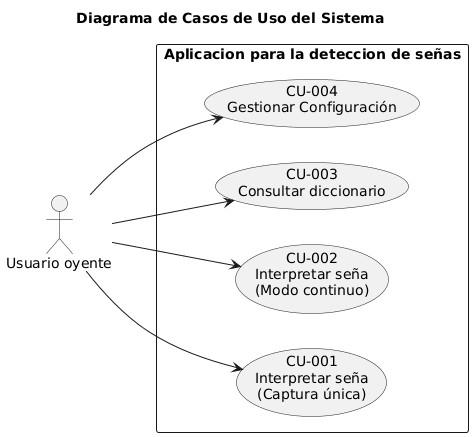
\includegraphics[width=0.6\textwidth]{images/fig24.jpg}
		\caption{Diagrama de Casos de Uso  LSM.}
		\label{fig:CU}
	\end{figure}
	
	\rowcolors{2}{rowblue}{white}
	
	\small
	\renewcommand{\arraystretch}{1.15}
	
	\begin{longtable}{|p{2.0cm}|p{3.5cm}|p{7.5cm}|p{2.0cm}|}
		\caption{Casos de uso del prototipo} \\
		\hline
		\rowcolor{headerblue}
		\headercell{ID} &
		\headercell{Nombre} &
		\headercell{Descripción} &
		\headercell{Actor principal} \\
		\hline
		\endfirsthead
		
		\hline
		\rowcolor{headerblue}
		\headercell{ID} &
		\headercell{Nombre} &
		\headercell{Descripción} &
		\headercell{Actor principal} \\
		\hline
		\endhead
		
		\rowcolors{1}{rowblue}{white}
		
		CU-001 &
		Interpretar seña (captura única) &
		El usuario captura una imagen de una seña estática mediante la cámara del dispositivo, con el objetivo de obtener su traducción en texto. &
		Usuario oyente \\
		\hline
		
		CU-002 &
		Interpretar seña (modo continuo) &
		El usuario utiliza la cámara del dispositivo para realizar una seña y el sistema ejecuta el reconocimiento de manera continua dentro del área de captura, mostrando la traducción detectada durante el proceso de inferencia. &
		Usuario oyente \\
		\hline
		
		CU-003 &
		Consultar diccionario de señas &
		El usuario navega por un conjunto de representaciones visuales de señas para aprender o verificar la forma correcta de realizarlas. &
		Usuario oyente \\
		\hline
		
		CU-004 &
		Gestionar configuración &
		El usuario accede a opciones de configuración para consultar información de uso o ajustar parámetros básicos de la aplicación. &
		Usuario oyente \\
		\hline
		
	\end{longtable}
	
	
	\subsubsection{Descripción detallada de casos de uso}
	
	\textbf{CU-001: Interpretar Seña (Captura Única)}
	
	\begin{itemize}
		
		\item \textbf{ID:} CU-001
		
		\item \textbf{Nombre:} Interpretar Seña (Captura Única)
		
		\item \textbf{Actor principal:} Usuario oyente
		
		\item \textbf{Descripción:} El usuario captura una imagen de una seña estática mediante la cámara del dispositivo. El sistema procesa la imagen, extrae las características relevantes, ejecuta el modelo de clasificación y muestra la traducción textual correspondiente.
		
		\item \textbf{Precondiciones:}
		\begin{enumerate}
			\item La aplicación se encuentra instalada en el dispositivo.
			\item El usuario ha concedido permisos de acceso a la cámara.
			\item El modelo de clasificación ha sido cargado correctamente en el sistema.
		\end{enumerate}
		
		\item \textbf{Resultado esperado:} El sistema muestra en pantalla la letra correspondiente a la seña capturada, junto con la opción de consultar información adicional en el diccionario.
		
	\end{itemize}
	
	
	\textbf{Flujo principal:}
	
	\begin{enumerate}
		\item El usuario inicia la aplicación o selecciona el modo ``Captura Única''.
		\item El sistema activa la cámara y muestra la vista previa.
		\item El usuario posiciona la seña dentro del área de captura y presiona el botón ``Capturar''.
		\item El sistema captura la imagen.
		\item El sistema procesa la imagen y extrae los puntos clave de la mano mediante MediaPipe.
		\item El sistema genera un vector de características a partir de los landmarks.
		\item El sistema ejecuta la inferencia utilizando el modelo de clasificación.
		\item El sistema genera una predicción con etiqueta y nivel de confianza.
		\item El sistema valida la confianza de la predicción (Regla RN-01).
		\item El sistema muestra la etiqueta reconocida en pantalla.
		\item El sistema habilita la opción de consultar la seña en el diccionario.
		
	\end{enumerate}
	
	\textbf{Trayectorias alternativas:}
	
	\begin{itemize}
		
		\item \textbf{A1: Predicción con baja confianza}
		\begin{itemize}
			\item \textbf{Condición:} En el paso 9, la confianza de la predicción es inferior al umbral definido.
			\item \textbf{Flujo:}
			\begin{enumerate}
				\item El sistema muestra un mensaje indicando que la seña no pudo ser reconocida.
			\end{enumerate}
		\end{itemize}
		
		\item \textbf{A2: Cancelación del usuario}
		\begin{itemize}
			\item \textbf{Condición:} En el paso 3, el usuario decide cancelar la operación.
			\item \textbf{Flujo:}
			\begin{enumerate}
				\item El sistema regresa a la pantalla principal.
			\end{enumerate}
		\end{itemize}
		
	\end{itemize}
	
	\begin{figure}[H]
		\centering
		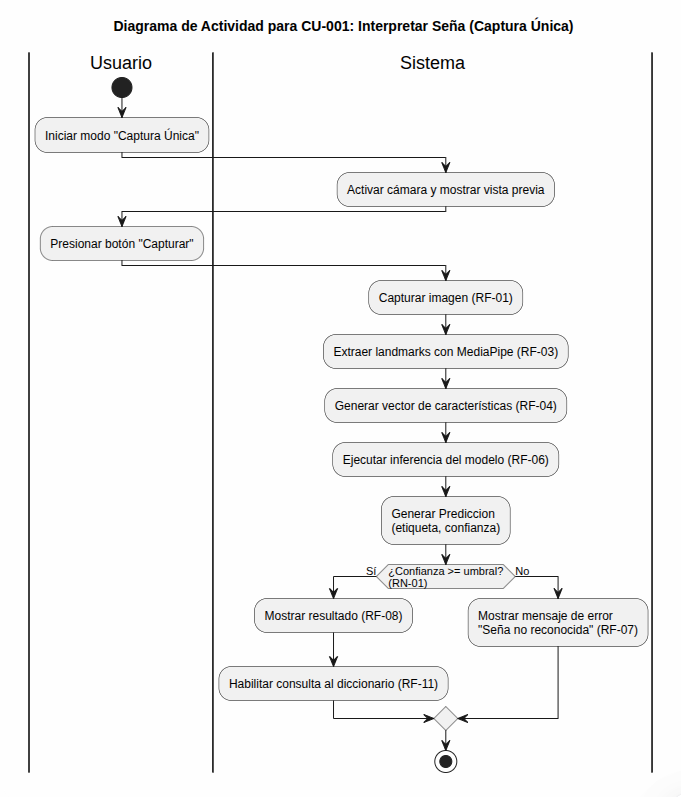
\includegraphics[width=0.7\textwidth]{images/fig25.png}
		\caption{Diagrama de actividades de CU-001}
		\label{fig:CU01}
	\end{figure}
	
	
	\textbf{CU-002: Interpretar Seña (Modo Continuo)}
	
	\begin{itemize}
		
		\item \textbf{ID:} CU-002
		
		\item \textbf{Nombre:} Interpretar Seña (Modo Continuo)
		
		\item \textbf{Actor principal:} Usuario oyente
		
		\item \textbf{Descripción:} El usuario apunta la cámara hacia una seña estática y el sistema realiza el reconocimiento de forma continua dentro del área de captura definida en la interfaz, mostrando en pantalla la traducción textual correspondiente.
		
		\item \textbf{Precondiciones:}
		\begin{enumerate}
			\item La aplicación se encuentra instalada en el dispositivo.
			\item El usuario ha concedido permisos de acceso a la cámara.
			\item El modelo de clasificación ha sido cargado correctamente en el sistema.
			\item El usuario ha seleccionado el modo de reconocimiento continuo.
		\end{enumerate}
		
		\item \textbf{Resultado esperado:} El sistema actualiza en pantalla la letra reconocida de manera continua mientras la seña permanezca dentro del área de captura y la confianza de la predicción sea válida.
		
	\end{itemize}
	
	\textbf{Flujo principal:}
	
	\begin{enumerate}
		\item El usuario selecciona el modo ``Iniciar Intérprete''.
		\item El sistema activa la cámara y muestra la vista previa junto con el área de captura.
		\item El sistema inicia el procesamiento continuo de fotogramas.
		\item El sistema obtiene el fotograma más reciente de la cámara.
		\item El sistema identifica la región de interés correspondiente al área de captura.
		\item El sistema extrae los landmarks de la mano mediante MediaPipe.
		\item El sistema genera un vector de características a partir de los landmarks.
		\item El sistema ejecuta la inferencia del modelo.
		\item El sistema genera una predicción con etiqueta y nivel de confianza.
		\item El sistema valida la confianza de la predicción (RN-01).
		\item El sistema actualiza el texto mostrado en pantalla con la etiqueta reconocida.
		\item El proceso se repite mientras el modo continuo permanezca activo.
		
	\end{enumerate}
	
	\textbf{Trayectorias alternativas:}
	
	\begin{itemize}
		
		\item \textbf{A1: Predicción con baja confianza}
		\begin{itemize}
			\item \textbf{Condición:} En el paso 10, la confianza de la predicción es inferior al umbral definido.
			\item \textbf{Flujo:}
			\begin{enumerate}
				\item El sistema muestra un indicador de reconocimiento no válido o limpia temporalmente el resultado en pantalla.
				\item El sistema continúa con el procesamiento del siguiente fotograma.
			\end{enumerate}
		\end{itemize}
		
		\item \textbf{A2: Salida del modo continuo}
		\begin{itemize}
			\item \textbf{Condición:} El usuario decide salir del modo de reconocimiento continuo.
			\item \textbf{Flujo:}
			\begin{enumerate}
				\item El sistema detiene la captura y el procesamiento de fotogramas.
				\item El sistema regresa a la pantalla principal o al menú anterior.
			\end{enumerate}
		\end{itemize}
		
	\end{itemize}
	
	\begin{figure}[H]
		\centering
		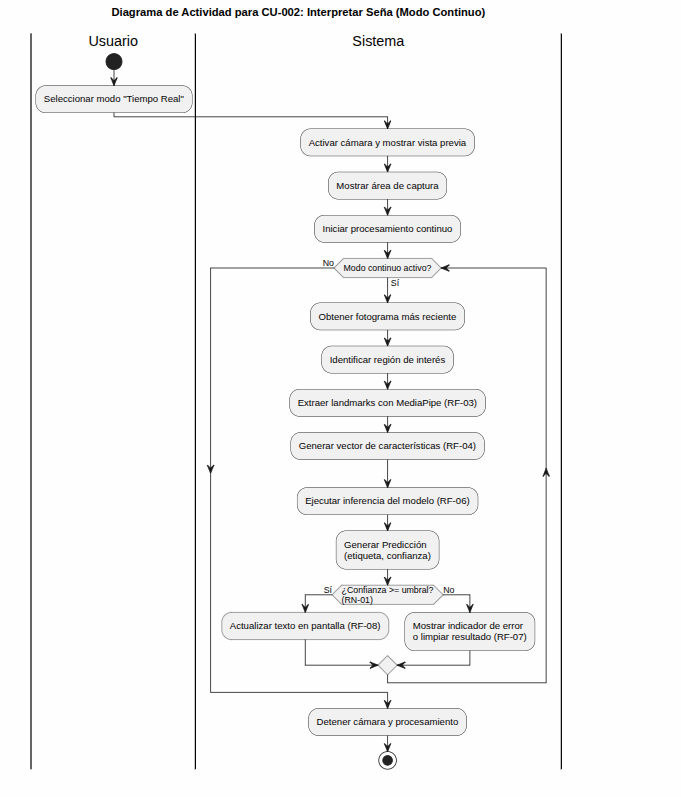
\includegraphics[width=0.9\textwidth]{images/fig26.png}
		\caption{Diagrama de actividades de CU-002}
		\label{fig:CU02}
	\end{figure}
	
	
	\textbf{CU-003: Consultar Diccionario de Señas}
	
	\begin{itemize}
		
		\item \textbf{ID:} CU-003
		
		\item \textbf{Nombre:} Consultar Diccionario de Señas
		
		\item \textbf{Actor principal:} Usuario oyente
		
		\item \textbf{Descripción:} El usuario consulta un conjunto de representaciones visuales de señas correspondientes al alfabeto de la Lengua de Señas Mexicana, con el fin de verificar la forma correcta de realizarlas (cumple RU-007).
		
		\item \textbf{Precondiciones:}
		\begin{enumerate}
			\item La aplicación se encuentra instalada en el dispositivo.
		\end{enumerate}
		
		\item \textbf{Resultado esperado:} El sistema muestra la representación visual de la seña seleccionada, junto con su descripción correspondiente.
		
	\end{itemize}
	
	\textbf{Flujo principal:}
	
	\begin{enumerate}
		\item El usuario accede a la sección ``Diccionario'' desde la interfaz principal.
		\item El sistema muestra una lista o cuadrícula con las señas disponibles.
		\item El usuario selecciona una seña específica (por ejemplo, ``C'').
		\item El sistema recupera la información correspondiente a la seña seleccionada.
		\item El sistema muestra la representación visual de la seña (imagen o animación) junto con su descripción.
		
	\end{enumerate}
	
	\textbf{Trayectorias alternativas:}
	
	\begin{itemize}
		
		\item \textbf{A1: Consulta desde predicción}
		\begin{itemize}
			\item \textbf{Condición:} El usuario ha obtenido previamente una predicción válida en los casos de uso CU-001 o CU-002.
			\item \textbf{Flujo:}
			\begin{enumerate}
				\item El sistema muestra el resultado junto con la opción de consultar la seña en el diccionario (RF-11).
				\item El usuario selecciona la opción de consulta.
				\item El sistema muestra directamente el detalle de la seña correspondiente.
			\end{enumerate}
		\end{itemize}
		
	\end{itemize}
	
	
	\begin{figure}[H]
		\centering
		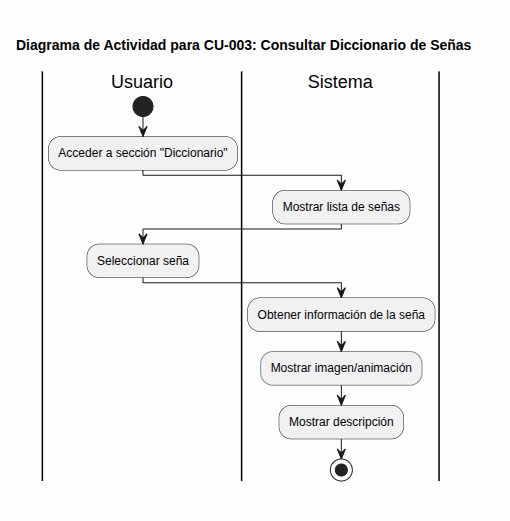
\includegraphics[width=0.7\textwidth]{images/fig27.png}
		\caption{Diagrama de actividades de CU-003}
		\label{fig:CU03}
	\end{figure}
	\newpage
	
	\textbf{CU-004: Gestionar configuración}
	
	\begin{itemize}
		
		\item \textbf{ID:} CU-004
		
		\item \textbf{Nombre:} Gestionar configuración
		
		\item \textbf{Actor principal:} Usuario oyente
		
		\item \textbf{Descripción:} El usuario accede a la sección de configuración de la aplicación para consultar información de uso o ajustar preferencias básicas del sistema.
		
		\item \textbf{Precondiciones:}
		\begin{enumerate}
			\item La aplicación se encuentra instalada en el dispositivo.
		\end{enumerate}
		
		\item \textbf{Resultado esperado:} El usuario puede consultar el tutorial de uso o modificar configuraciones disponibles dentro de la aplicación.
		
	\end{itemize}
	
	\textbf{Flujo principal (consulta de tutorial):}
	
	\begin{enumerate}
		\item El usuario accede a la opción ``Configuración'' desde la pantalla principal.
		\item El sistema muestra la pantalla de configuración.
		\item El usuario selecciona la opción ``Ver tutorial''.
		\item El sistema muestra una guía de uso de la aplicación (pantallas informativas o contenido multimedia).
	\end{enumerate}
	
	\textbf{Trayectorias alternativas:}
	
	\begin{itemize}
		
		\item \textbf{A1: Modificación de preferencias}
		\begin{itemize}
			\item \textbf{Condición:} El usuario selecciona una opción de configuración distinta al tutorial.
			\item \textbf{Flujo:}
			\begin{enumerate}
				\item El usuario selecciona una preferencia disponible.
				\item El sistema aplica el cambio correspondiente.
			\end{enumerate}
		\end{itemize}
		
		\item \textbf{A2: Salida de configuración}
		\begin{itemize}
			\item \textbf{Condición:} El usuario decide salir de la sección de configuración.
			\item \textbf{Flujo:}
			\begin{enumerate}
				\item El sistema regresa a la pantalla principal.
			\end{enumerate}
		\end{itemize}
		
	\end{itemize}
	
	\begin{figure}[H]
		\centering
		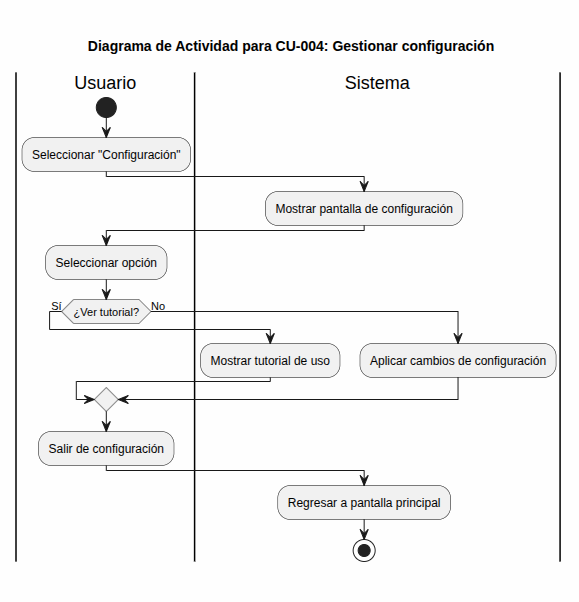
\includegraphics[width=0.7\textwidth]{images/fig28.png}
		\caption{Diagrama de actividades de CU-004}
		\label{fig:CU04}
	\end{figure}
	
	\subsection{Análisis de riesgos}
	
	El análisis de riesgos es algo importante dentro del proceso de diseño, ya que permite identificar, evaluar y mitigar los eventos que pueden comprometer la calidad, funcionalidad o cumplimiento de los objetivos del sistema. De acuerdo con la norma internacional ISO 31000 para la gestión de riesgos, el análisis debe realizarse de manera anticipada al diseño detallado, con el fin de establecer medidas de control oportunas \cite{iso31000}. El estándar IEEE 12207 señala que la gestión de riesgos debe mantenerse a lo largo de todo el ciclo de vida del software \cite{ieee12207}.
	
	En el presente proyecto, los riesgos se agrupan en cuatro categorías principales: riesgos técnicos, riesgos de datos, riesgos de integración y riesgos operativos. En aplicaciones de visión por computadora, la literatura indica que el desempeño del sistema depende en gran medida de la calidad y representatividad de los datos utilizados en el entrenamiento \cite{goodfellow2016}.
	
	Un riesgo técnico relevante es el sobreajuste del modelo, específicamente cuando el conjunto de datos no representa adecuadamente las condiciones reales de uso. Este fenómeno puede provocar que el sistema aprenda patrones no generalizables, como condiciones específicas de iluminación o características del entorno. Para mitigar este riesgo, se emplean técnicas de validación y variación en las condiciones de captura.
	
	Otro riesgo técnico importante está asociado a la detección de la mano mediante MediaPipe. Dado que el sistema depende de la correcta extracción de landmarks, fallos en la detección —provocados por iluminación deficiente, oclusiones o posicionamiento incorrecto de la mano— pueden impedir el reconocimiento adecuado de la seña. Este riesgo se reduce mediante el uso de guías visuales en la interfaz y la validación de condiciones mínimas de captura.
	
	En cuanto a los riesgos de datos, la falta de variabilidad en el conjunto de entrenamiento puede afectar la capacidad del modelo para generalizar. Como señala Szeliski, los sistemas de visión deben considerar variaciones en pose, escala e iluminación para evitar comportamientos frágiles \cite{szeliski2010}. Para mitigar este riesgo, se incorporan muestras diversas y se evalúa el modelo en diferentes condiciones.
	
	Un riesgo adicional corresponde a la inconsistencia entre el procesamiento de datos en la etapa de entrenamiento y la etapa de inferencia. Diferencias en la normalización o en la forma de representar los datos pueden degradar significativamente el desempeño del modelo. Para evitar este problema, se define un pipeline de procesamiento uniforme en ambas etapas.
	
	En el entorno móvil, existen riesgos relacionados con el rendimiento del sistema, tales como latencias elevadas o consumo excesivo de recursos. Aunque el modelo utilizado es ligero, las limitaciones del hardware pueden afectar la experiencia del usuario. Para mitigar este riesgo, se prioriza el uso de modelos eficientes y se realizan pruebas en dispositivos reales.
	
	Como último paso se consideran riesgos operativos relacionados con el tiempo de desarrollo, disponibilidad de recursos computacionales y complejidad en la evaluación del modelo. Estos riesgos se abordan mediante una planificación adecuada y la utilización de herramientas optimizadas para el entrenamiento y validación.
	
	El análisis de riesgos permite priorizar los factores que pueden afectar el desempeño del sistema y establecer estrategias de mitigación adecuadas. En la siguiente sección se presenta la tabla de riesgos, donde se clasifican de acuerdo con su probabilidad, impacto y acciones de control.
	
	\rowcolors{2}{rowblue}{white}
	
	\small
	\renewcommand{\arraystretch}{1.15}
	
	\begin{longtable}{|p{1.2cm}|p{4.2cm}|p{1.5cm}|p{1.5cm}|p{1.5cm}|p{4.5cm}|}
		\caption{Tabla de riesgos del proyecto} \\
		\hline
		\rowcolor{headerblue}
		\headercell{ID} &
		\headercell{Riesgo} &
		\headercell{Prob.} &
		\headercell{Impacto} &
		\headercell{Nivel} &
		\headercell{Mitigación} \\
		\hline
		\endfirsthead
		
		\hline
		\rowcolor{headerblue}
		\headercell{ID} &
		\headercell{Riesgo} &
		\headercell{Prob.} &
		\headercell{Impacto} &
		\headercell{Nivel} &
		\headercell{Mitigación} \\
		\hline
		\endhead
		
		\rowcolors{1}{rowblue}{white}
		
		R1 &
		Sobreajuste del modelo por baja variabilidad del dataset &
		Media &
		Alto &
		Alto &
		Aumento de datos, validación cruzada y diversidad de condiciones de captura \\
		\hline
		
		R2 &
		Inconsistencia entre procesamiento en entrenamiento e inferencia &
		Baja &
		Alto &
		Medio &
		Definir un pipeline de procesamiento unificado \\
		\hline
		
		R3 &
		Latencia elevada en la ejecución del modelo en dispositivos móviles &
		Media &
		Alto &
		Alto &
		Uso de modelos ligeros y pruebas de rendimiento en dispositivo \\
		\hline
		
		R4 &
		Pérdida de precisión del modelo en entorno real &
		Media &
		Medio &
		Medio &
		Evaluación en condiciones reales y ajuste del modelo \\
		\hline
		
		R5 &
		Limitaciones de hardware en dispositivos de gama baja &
		Media &
		Alto &
		Alto &
		Optimización del modelo y pruebas en distintos dispositivos \\
		\hline
		
		R6 &
		Errores en el procesamiento de imagen capturada &
		Media &
		Medio &
		Medio &
		Validación de entrada y pruebas con distintos formatos de imagen \\
		\hline
		
		R7 &
		Desbalance de clases en el dataset &
		Baja &
		Medio &
		Bajo &
		Balanceo de datos y muestreo controlado \\
		\hline
		
		R8 &
		Variabilidad en iluminación durante la captura &
		Alta &
		Medio &
		Alto &
		Aumento de datos y pruebas en diferentes condiciones de luz \\
		\hline
		
		R9 &
		Oclusión o mala posición de la mano &
		Media &
		Medio &
		Medio &
		Guías visuales y dataset con mayor variabilidad \\
		\hline
		
		R10 &
		Errores en orientación o rotación de la imagen &
		Media &
		Medio &
		Medio &
		Corrección automática mediante herramientas del sistema \\
		\hline
		
		R11 &
		Fallos en integración entre modelo y aplicación móvil &
		Baja &
		Alto &
		Medio &
		Pruebas de integración y validación continua \\
		\hline
		
		R12 &
		Incompatibilidad entre versiones de librerías &
		Baja &
		Alto &
		Medio &
		Control de versiones y pruebas regresivas \\
		\hline
		
		R13 &
		Consumo energético elevado en modo continuo &
		Media &
		Medio &
		Medio &
		Optimización de frecuencia de procesamiento \\
		\hline
		
		R14 &
		Limitaciones de memoria en el dispositivo &
		Baja &
		Alto &
		Medio &
		Carga eficiente del modelo y control de recursos \\
		\hline
		
		R15 &
		Tiempos elevados de entrenamiento del modelo &
		Media &
		Bajo &
		Bajo &
		Uso de hardware acelerado y optimización de entrenamiento \\
		\hline
		
		R16 &
		Costo computacional de validación del modelo &
		Media &
		Medio &
		Medio &
		Uso de validaciones reducidas en etapas iniciales \\
		\hline
		
		R17 &
		Baja interpretabilidad del resultado para el usuario &
		Baja &
		Bajo &
		Bajo &
		Mostrar resultados claros y nivel de confianza \\
		\hline
		
		R18 &
		Dependencia de condiciones de fondo durante la captura &
		Media &
		Medio &
		Medio &
		Aumento de datos con fondos variados \\
		\hline
		
		R19 &
		Falta de estandarización en la captura del usuario &
		Alta &
		Medio &
		Alto &
		Uso de guías visuales en pantalla (ROI) \\
		\hline
		
		R20 &
		Fallas en la detección de la mano (MediaPipe) &
		Media &
		Alto &
		Alto &
		Optimización de condiciones de captura y validación de detección \\
		\hline
		
		R21 &
		Problemas de compatibilidad de cámara entre dispositivos &
		Media &
		Alto &
		Alto &
		Uso de APIs estándar como CameraX \\
		\hline
		
	\end{longtable}
	Aunque el PMBOK propone matrices de probabilidad e impacto basadas en escalas cuantitativas, el propio estándar establece que las herramientas de análisis deben adaptarse al tamaño, alcance y nivel de complejidad del proyecto. En este sentido, el PMBOK 7 indica que los equipos pueden simplificar o ampliar los métodos de evaluación de riesgos de acuerdo con su contexto organizacional, incluyendo el uso de escalas cualitativas cuando no se requieren mediciones numéricas detalladas \cite{pmbok2021}.
	
	De manera complementaria, la norma ISO 31000 señala que las escalas utilizadas en el análisis de riesgos deben ser adecuadas al contexto y al nivel de detalle requerido para la toma de decisiones \cite{iso31000}.
	
	Con base en lo anterior, en el presente proyecto se adopta una matriz cualitativa de probabilidad e impacto de tipo 3×3 (Bajo, Medio, Alto), la cual mantiene consistencia conceptual con los estándares internacionales, al mismo tiempo que resulta proporcional al alcance y complejidad del sistema desarrollado.
	
	\begin{figure}[H]
		\centering
		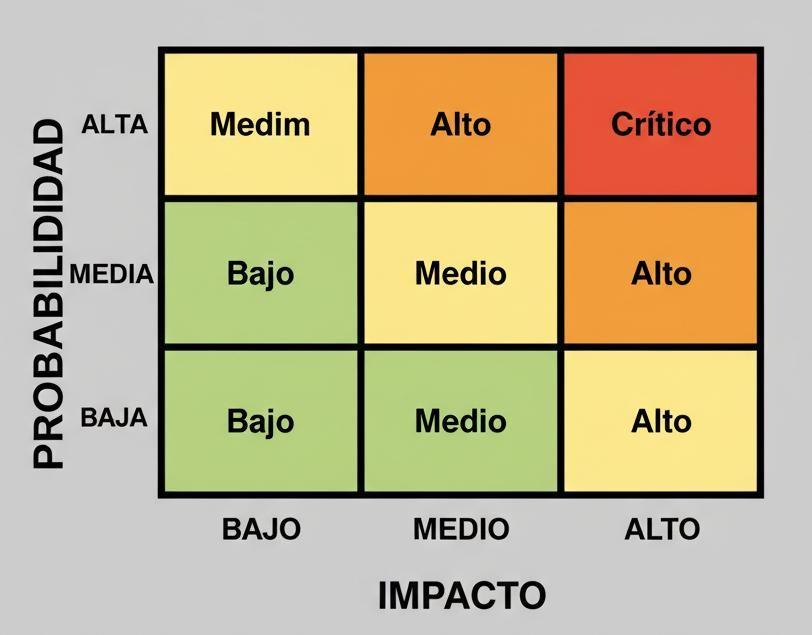
\includegraphics[width=0.4\textwidth]{images/fig29.jpg}
		\caption{Matriz de probabilidad-impacto para la evaluación de riesgos del proyecto }
		\label{fig:riesgos}
	\end{figure}
	
	La Figura 28 presenta la matriz de probabilidad–impacto utilizada para evaluar y priorizar los riesgos identificados en el proyecto. Este tipo de matriz es una herramienta ampliamente utilizada en la gestión de riesgos, recomendada tanto por el PMBOK 7 como por la norma ISO 31000, ya que permite visualizar de manera clara la severidad de cada riesgo en función de dos dimensiones fundamentales: la probabilidad de ocurrencia y el impacto potencial sobre los objetivos del proyecto \cite{iso31000,pmbok2021}.
	
	De acuerdo con ISO 31000, el análisis de riesgos debe emplear escalas adecuadas al contexto y al nivel de detalle requerido, permitiendo el uso de enfoques cualitativos cuando no se requieren mediciones cuantitativas avanzadas \cite{iso31000}. En este sentido, la matriz utilizada en este proyecto adopta un esquema cualitativo de tipo 3×3 (Bajo, Medio, Alto), consistente con la tabla de riesgos presentada previamente y proporcional al alcance del sistema desarrollado.
	
	La probabilidad se clasifica en tres niveles:
	\begin{itemize}
		\item \textbf{Alta:} el riesgo es muy probable o recurrente.
		\item \textbf{Media:} existe una probabilidad moderada de ocurrencia.
		\item \textbf{Baja:} el evento es poco probable.
	\end{itemize}
	
	De manera similar, el impacto se categoriza como:
	\begin{itemize}
		\item \textbf{Alto:} afecta el funcionamiento del sistema, los entregables principales o los tiempos del proyecto.
		\item \textbf{Medio:} genera afectaciones parciales o retrasos moderados.
		\item \textbf{Bajo:} su efecto sobre el proyecto es mínimo.
	\end{itemize}
	
	Cada celda de la matriz representa la combinación de estos factores, permitiendo clasificar los riesgos según su nivel de severidad. Para facilitar su interpretación, se utiliza una codificación cromática común en mapas de riesgo, donde cada color indica el nivel de prioridad de atención \cite{riskheatmap}:
	
	\begin{itemize}
		\item \textbf{Verde:} riesgo bajo, aceptable y sin necesidad de acciones inmediatas.
		\item \textbf{Amarillo:} riesgo medio, requiere monitoreo y acciones preventivas.
		\item \textbf{Naranja:} riesgo alto, requiere mitigación prioritaria.
		\item \textbf{Rojo:} riesgo crítico, requiere atención inmediata.
	\end{itemize}
	
	Este esquema visual permite identificar de manera clara los riesgos que deben atenderse con mayor prioridad, como aquellos relacionados con la detección de la mano, el rendimiento en dispositivos móviles o la consistencia del procesamiento de datos. De esta forma, la matriz facilita la toma de decisiones y complementa el análisis presentado en la tabla de riesgos.
	
	
	\subsection{Costos del proyecto}
	
	
	El presente trabajo corresponde al desarrollo de un prototipo experimental orientado a la validación de una solución tecnológica, y no a la implementación de un producto comercial en producción. Por esta razón, los costos presentados en esta sección no representan una cotización real de despliegue industrial, sino una estimación académica basada en el modelo COCOMO II, la cual permite dimensionar el esfuerzo humano y los recursos tecnológicos involucrados en el desarrollo del proyecto.
	
	De acuerdo con el estándar IEEE 12207, la estimación de costos en proyectos de software tiene como finalidad analizar la viabilidad, estimar el esfuerzo de ingeniería y documentar el proceso de desarrollo, sin implicar necesariamente una implementación comercial \cite{ieee12207}. La literatura en ingeniería de software establece que la estimación debe considerar tanto el esfuerzo humano como los recursos materiales y tecnológicos utilizados a lo largo del ciclo de vida del sistema. De forma complementaria, el PMBOK recomienda incluir tanto costos tangibles como intangibles para obtener una visión integral del proyecto \cite{pmbok2021}.
	Esta sección tiene como objetivo estimar el costo total asociado al desarrollo del prototipo, considerando los recursos de hardware, software y el tiempo de dedicación requerido para su implementación.
	
	El desarrollo del prototipo se realizara en una computadora portátil Lenovo Legion 7 Pro equipada con una GPU NVIDIA RTX 4090 Laptop, cuya capacidad de cómputo resulta adecuada para el procesamiento de datos, entrenamiento de modelos y experimentación. La depreciación del equipo se estima con base en su vida útil y el tiempo de uso en el proyecto. Asimismo, se emplea un dispositivo móvil Poco F7 Pro y una tablet Lenovo yoga tab plus para la validación del modelo en entorno Android, particularmente en pruebas de reconocimiento continuo.
	
	A continuación, se presenta la estimación de costos del proyecto, desglosada por tipo de recurso y esfuerzo involucrado.
	
	\rowcolors{2}{rowblue}{white}
	
	\small
	\renewcommand{\arraystretch}{1.15}
	
	\begin{longtable}{|p{9cm}|p{4cm}|}
		\caption{Costos del equipo utilizado para el desarrollo del proyecto} \\
		\hline
		\rowcolor{headerblue}
		\headercell{Recurso} &
		\headercell{Costo total estimado} \\
		\hline
		\endfirsthead
		
		\hline
		\rowcolor{headerblue}
		\headercell{Recurso} &
		\headercell{Costo total estimado} \\
		\hline
		\endhead
		
		\rowcolors{1}{rowblue}{white}
		
		Laptop Lenovo Legion 7 Pro &
		\$83,000 MXN \\
		\hline
		
		Teléfono Poco F7 Pro &
		\$9,000 MXN \\
		\hline
		
		Accesorios (trípode, iluminación) &
		\$1,000 MXN \\
		\hline
		
	\end{longtable}
	\textbf{Total de costos del equipo: \$ 93,000 MXN }
	
	Aunque todo el software empleado es libre (Android Studio, TensorFlow, Python, NumPy, TFLite), se considera el costo indirecto de servicios necesarios para operar el prototipo, como conexión a internet de alta velocidad. 
	
	\rowcolors{2}{rowblue}{white}
	
	\small
	\renewcommand{\arraystretch}{1.15}
	\arrayrulecolor{black}
	\begin{longtable}{|p{9cm}|p{4cm}|}
		\caption{Costos de software y servicios utilizados en el proyecto} \\
		\hline
		\rowcolor{headerblue}
		\headercell{Rubro} &
		\headercell{Costo} \\
		\hline
		\endfirsthead
		
		\hline
		\rowcolor{headerblue}
		\headercell{Rubro} &
		\headercell{Costo} \\
		\hline
		\endhead
		
		\rowcolors{1}{rowblue}{white}
		
		Internet (9 meses $\times$ \$500 MXN/mes) &
		\$4{,}500 MXN \\
		\hline
		
		Software libre y licencias &
		\$0 MXN \\
		\hline
		
	\end{longtable}
	
	El prototipo se desarrollará utilizando una laptop Lenovo Legion 7 Pro con un adaptador de corriente de 330 W, la cual se mantendrá activa durante sesiones de experimentación y entrenamiento. La la laptop será utilizada al menos 5 horas diarias durante un periodo aproximado de 9 meses, lo que representa una parte significativa del costo energético del proyecto. 
	El cálculo se realizó con base en el costo promedio nacional por kWh establecido por la Comisión Federal de Electricidad (CFE), equivalente a \$1.10 MXN por kWh. El consumo total estimado se obtiene de la siguiente manera:
	
	\begin{itemize}
		
		\item \textbf{Consumo del equipo:}  
		330 W = 0.33 kW
		
		\item \textbf{Uso mensual:}  
		5 horas diarias $\times$ 30 días = 150 horas/mes
		
		\item \textbf{Uso total (9 meses):}  
		150 $\times$ 9 = 1,350 horas
		
		\item \textbf{Energía consumida:}  
		0.33 kW $\times$ 1,350 h = 445.5 kWh
		
		\item \textbf{Costo total:}  
		\textbf{445.5 kWh $\times$ 1.1 MXN = 490.05 MXN}
		
	\end{itemize} 
	
	La capacitación técnica requerida para el desarrollo del prototipo representa un costo imputable al proyecto, conforme a los lineamientos de formación y adquisición de competencias establecidos en IEEE 12207, así como a las recomendaciones de estimación de costos del PMBOK \cite{ieee12207,pmbok2021}. 
	
	Aunque el desarrollo fue realizado por un solo integrante, fue necesario adquirir conocimientos especializados en procesamiento de imágenes, aprendizaje automático, uso de MediaPipe para la extracción de características de la mano, implementación de modelos en TensorFlow Lite y desarrollo de aplicaciones móviles en Android Studio, incluyendo el uso de CameraX para la captura de imágenes.
	
	Estas actividades representan un total de 87 horas de capacitación técnica. Considerando un costo estimado de \$120 MXN por hora, se obtiene un costo total de \textbf{\$10,440 MXN}. Este valor refleja la inversión en formación necesaria para el desarrollo e implementación del prototipo.
	\rowcolors{2}{rowblue}{white}
	
	\small
	\renewcommand{\arraystretch}{1.15}
	
	\begin{longtable}{|p{5cm}|p{2.2cm}|p{2.5cm}|p{2.5cm}|}
		\caption{Costos de capacitación técnica del proyecto} \\
		\hline
		\rowcolor{headerblue}
		\headercell{Área de capacitación} &
		\headercell{Horas estimadas} &
		\headercell{Costo por hora (MXN)} &
		\headercell{Costo total (MXN)} \\
		\hline
		\endfirsthead
		
		\hline
		\rowcolor{headerblue}
		\headercell{Área de capacitación} &
		\headercell{Horas estimadas} &
		\headercell{Costo por hora (MXN)} &
		\headercell{Costo total (MXN)} \\
		\hline
		\endhead
		
		\rowcolors{1}{rowblue}{white}
		
		Modelos de aprendizaje automático &
		15 &
		120 &
		\$1{,}800 \\
		\hline
		
		TensorFlow / Keras &
		12 &
		120 &
		\$1{,}440 \\
		\hline
		
		TensorFlow Lite (optimización y conversión) &
		10 &
		120 &
		\$1{,}200 \\
		\hline
		
		Preprocesamiento de datos e imágenes &
		8 &
		120 &
		\$960 \\
		\hline
		
		Android Studio -- CameraX &
		14 &
		120 &
		\$1{,}680 \\
		\hline
		
		Android Studio -- ML / TFLite &
		12 &
		120 &
		\$1{,}440 \\
		\hline
		
		MediaPipe Hands &
		10 &
		120 &
		\$1{,}200 \\
		\hline
		
		Gestión de riesgos / COCOMO II &
		6 &
		120 &
		\$720 \\
		\hline
		
		\rowcolor{headerblue}
		\multicolumn{3}{|r|}{\textbf{Total}} &
		\textbf{\$10{,}440 MXN} \\
		\hline
		
	\end{longtable}
	
	\textbf{Total de capacitación: \$10,440 MXN }
	
	
	La estimación del esfuerzo humano es el componente central del costo total del prototipo, dado que en proyectos de ingeniería de software la mayor parte del gasto se asocia al tiempo de desarrollo y no a los recursos materiales. Boehm señala que entre el 60\% y 80\% del costo total de un sistema de software corresponde al esfuerzo humano invertido en actividades como análisis, diseño, implementación y pruebas \cite{boehm2000}.
	
	De acuerdo con el estándar IEEE 12207, incluso en sistemas de carácter experimental o prototipos, es necesario cuantificar el esfuerzo requerido en cada etapa del ciclo de vida del software, con el fin de garantizar la trazabilidad del proceso, documentar la complejidad del desarrollo y evaluar la viabilidad de la solución \cite{ieee12207}.
	
	Para este proyecto se emplea el modelo COCOMO II, el cual permite estimar el esfuerzo en términos de meses-persona a partir del tamaño del software y de factores asociados a la complejidad técnica. Dado que el prototipo integra procesamiento de imágenes, modelos de aprendizaje automático, optimización para ejecución en dispositivos móviles mediante TensorFlow Lite y el desarrollo de una aplicación Android, se clasifica como un proyecto de tipo \textit{Semidetached}, de acuerdo con la clasificación propuesta por Boehm para sistemas con complejidad intermedia y componentes heterogéneos \cite{boehm2000}.
	
	El tamaño del software se estimó considerando todos los componentes del prototipo, incluyendo scripts de procesamiento y entrenamiento, generación de características, pruebas experimentales, integración del modelo en el entorno móvil y desarrollo de la interfaz en Android Studio. Esta estimación permite establecer una base cuantitativa para el cálculo del esfuerzo total requerido en el proyecto.
	
	\rowcolors{2}{rowblue}{white}
	
	\small
	\renewcommand{\arraystretch}{1.15}
	
	\begin{longtable}{|p{9cm}|p{4cm}|}
		\caption{Estimación del tamaño del software del proyecto} \\
		\hline
		\rowcolor{headerblue}
		\headercell{Componente} &
		\headercell{LOC estimadas} \\
		\hline
		\endfirsthead
		
		\hline
		\rowcolor{headerblue}
		\headercell{Componente} &
		\headercell{LOC estimadas} \\
		\hline
		\endhead
		
		\rowcolors{1}{rowblue}{white}
		
		Procesamiento y entrenamiento en Python &
		1{,}500 \\
		\hline
		
		Integración TFLite + MediaPipe &
		800 \\
		\hline
		
		Aplicación Android (CameraX, interfaz e inferencia) &
		2{,}000 \\
		\hline
		
		Utilidades y scripts complementarios &
		700 \\
		\hline
		
		\rowcolor{headerblue}
		\textbf{Total estimado} &
		\textbf{5{,}000 LOC ($\approx$ 5 KLOC)} \\
		\hline
		
	\end{longtable}
	
	
	Entonces el valor seleccionado para el modelo COCOMO II es $KLOC = 5$. Este análisis requiere la definición de tres parámetros fundamentales: el tamaño del software ($KLOC$), el exponente de escala ($E$) y el factor de ajuste de esfuerzo ($EAF$).
	
	El exponente de escala se establece como $E = 1.03$. De acuerdo con Boehm, los proyectos que presentan una arquitectura parcialmente definida, son desarrollados por equipos pequeños o individuales, tienen complejidad técnica intermedia y riesgos moderadamente controlados, suelen ubicarse en un rango de $E$ entre 1.02 y 1.05 \cite{boehm2000}. Por lo tanto, la selección de $E = 1.03$ es consistente con la clasificación \textit{Semidetached} y con la naturaleza experimental del prototipo.
	
	El factor de ajuste de esfuerzo se define como $EAF = 1.05$. Este valor se obtiene a partir de la evaluación de los principales factores de costo (\textit{cost drivers}), considerando las características específicas del proyecto, tales como la complejidad del sistema, el tamaño del conjunto de datos, las restricciones de ejecución en dispositivos móviles y el uso de herramientas especializadas. En conjunto, estos factores ubican el proyecto dentro de un rango típico de $EAF$ entre 0.9 y 1.1, por lo que el valor seleccionado resulta adecuado.
	
	El cálculo del esfuerzo se realiza utilizando la expresión básica del modelo COCOMO II:
	
	\[
	PM = 2.94 \times (KLOC)^{E} \times EAF
	\]
	
	Sustituyendo los valores obtenidos:
	
	\[
	PM = 2.94 \times (5)^{1.03} \times 1.05 \approx 7.2 \ \text{meses-persona}
	\]
	
	La equivalencia entre meses-persona y horas de trabajo se ajusta considerando el contexto académico del proyecto. Aunque COCOMO II establece que un mes-persona puede oscilar entre 150 y 170 horas, en este trabajo se adopta una equivalencia de 100 horas por mes-persona, lo cual es coherente con la disponibilidad de tiempo. \cite{boehm2000,ieee12207,pmbok2021}.
	
	A partir de esta equivalencia, el esfuerzo total en horas se calcula como:
	
	\[
	7.2 \times 100 = 720 \ \text{horas}
	\]
	
	Finalmente considerando un costo de \$120 MXN por hora de desarrollo, el costo total del esfuerzo humano se estima como:
	
	\[
	720 \times 120 = \mathbf{86{,}400 \ \text{MXN}}
	\]
	
	\newpage
	\rowcolors{2}{rowblue}{white}
	
	\small
	\renewcommand{\arraystretch}{1.15}
	
	\begin{longtable}{|p{9cm}|p{4cm}|}
		\caption{Resumen del análisis de costos mediante el modelo COCOMO II} \\
		\hline
		\rowcolor{headerblue}
		\headercell{Concepto} &
		\headercell{Valor} \\
		\hline
		\endfirsthead
		
		\hline
		\rowcolor{headerblue}
		\headercell{Concepto} &
		\headercell{Valor} \\
		\hline
		\endhead
		
		\rowcolors{1}{rowblue}{white}
		
		Tamaño del software (KLOC) &
		5 \\
		\hline
		
		Esfuerzo estimado (COCOMO II) &
		7.2 meses-persona \\
		\hline
		
		Equivalencia por mes-persona &
		100 horas \\
		\hline
		
		Horas totales de desarrollo &
		720 horas \\
		\hline
		
		Tarifa por hora &
		\$120 MXN \\
		\hline
		
		\rowcolor{headerblue}
		\textbf{Costo humano total} &
		\textbf{\$86{,}400 MXN} \\
		\hline
		
	\end{longtable}
	
	\rowcolors{2}{rowblue}{white}
	
	\small
	\renewcommand{\arraystretch}{1.15}
	
	\begin{longtable}{|p{9cm}|p{4cm}|}
		\caption{Resumen general de costos del proyecto} \\
		\hline
		\rowcolor{headerblue}
		\headercell{Categoría} &
		\headercell{Costo} \\
		\hline
		\endfirsthead
		
		\hline
		\rowcolor{headerblue}
		\headercell{Categoría} &
		\headercell{Costo} \\
		\hline
		\endhead
		
		\rowcolors{1}{rowblue}{white}
		
		Equipo (hardware) &
		\$93{,}000 MXN \\
		\hline
		
		Servicios (internet y software) &
		\$4{,}500 MXN \\
		\hline
		
		Consumo eléctrico &
		\$490 MXN \\
		\hline
		
		Capacitación técnica &
		\$10{,}440 MXN \\
		\hline
		
		Costo humano (COCOMO II) &
		\$86{,}400 MXN \\
		\hline
		
		\rowcolor{headerblue}
		\textbf{Costo total del proyecto} &
		\textbf{\$194{,}830 MXN} \\
		\hline
		
	\end{longtable}
	\subsection{Arquitectura del sistema}
	
	
	La arquitectura del sistema propuesto se basa en un enfoque de procesamiento completamente local, en el cual el dispositivo móvil es responsable de ejecutar todas las etapas necesarias para la captura, el preprocesamiento, la clasificación y la visualización de la seña reconocida. Este enfoque permite mantener tiempos de respuesta reducidos en el proceso de reconocimiento, así como operar sin dependencia de conexión a internet, favoreciendo su disponibilidad en distintos contextos de uso.
	
	La ejecución local del procesamiento contribuye a mejorar la privacidad de la información del usuario, ya que no es necesario transmitir datos hacia servidores externos. Estas características permiten ofrecer una experiencia de uso fluida, eficiente y adecuada para aplicaciones de reconocimiento continuo orientadas a dispositivos móviles.
	
	Este enfoque podría funcionar para sistemas de reconocimiento gestual con procesamiento continuo, donde la velocidad de respuesta y la eficiencia computacional representan factores fundamentales para garantizar un funcionamiento estable en dispositivos móviles.
	
	\begin{figure}[H]
		\centering
		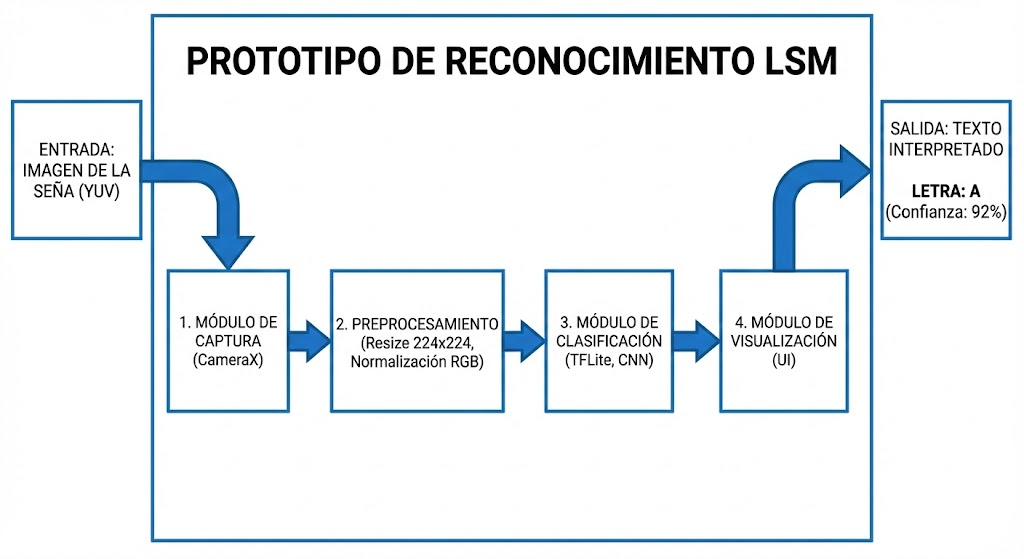
\includegraphics[width=0.8\textwidth]{images/fig30.png}
		\caption{Arquitectura del prototipo.}
		\label{fig:arquitectura}
	\end{figure}
	
	El prototipo se estructura en cuatro módulos principales:
	
	\textbf{Módulo de captura.}  
	
	Es el punto de entrada del sistema y es responsable de obtener los fotogramas provenientes del hardware de la cámara del dispositivo móvil. Para ello, se emplea la API CameraX, la cual permite una captura estable, compatible con múltiples dispositivos Android.
	
	El módulo de captura permite la adquisición de imágenes tanto en modo continuo como en modo controlado por el usuario, proporcionando flexibilidad en la operación del sistema. En la ejecución la cámara genera un flujo constante de fotogramas que representa la entrada visual del sistema, a partir de la cual se llevarán a cabo las etapas posteriores de procesamiento y reconocimiento.
	
	En los sistemas Android modernos, la cámara no entrega imágenes directamente en formato RGB, sino que proporciona los fotogramas en el formato \texttt{YUV\_420\_888}, el cual corresponde al formato estándar definido en la API Camera2 para la recepción de datos crudos del sensor. Este formato separa la información en componentes de luminancia (Y) y crominancia (U, V), lo que permite una representación más eficiente en términos de memoria y ancho de banda \cite{android_yuv,opencv_yuv}.
	
	La elección de este formato no es arbitraria, ya que los sensores de imagen capturan principalmente información de intensidad luminosa, y el modelo YUV permite una codificación del color más compacta sin afectar significativamente la percepción visual. En visión por computadora, este tipo de representación resulta adecuada para transmisión y procesamiento de video en continua debido a su eficiencia computacional \cite{gonzalez2002digital}.
	
	Aunque el formato YUV es óptimo a nivel de hardware, no siempre es directamente compatible con las bibliotecas de aprendizaje automático. En este proyecto, dependiendo de la etapa del pipeline, los fotogramas pueden ser transformados o utilizados de manera indirecta para facilitar su procesamiento. En particular, el sistema no realiza la clasificación directamente sobre la imagen completa, sino que emplea un enfoque basado en la detección de la mano y la extracción de características estructurales mediante landmarks.
	
	El módulo de captura no solo se limita a obtener los fotogramas, sino que debe garantizar que estos presenten una calidad y estabilidad suficientes para permitir una detección confiable por parte de MediaPipe. Esto incluye aspectos como iluminación adecuada, resolución controlada y consistencia temporal entre fotogramas.
	
	La cámara genera un flujo continuo de imágenes similar a un video. El módulo de captura selecciona siempre el fotograma más reciente disponible, ya que evita la acumulación de imágenes en memoria y reduce la latencia del sistema \cite{camerax_doc}.
	
	FPor ultimo la salida de este módulo consiste en la entrega de fotogramas actualizados que sirven como entrada para el módulo de procesamiento, en el cual se realizará la detección de la mano y la extracción de landmarks que es la base para la posterior clasificación de la seña.
	
	\textbf{Módulo de preprocesamiento.}  
	
	Recibe la información proveniente del módulo de captura y la transforma en una representación numérica adecuada para su procesamiento por el modelo de clasificación. A diferencia de enfoques tradicionales basados en imágenes completas, en este sistema el preprocesamiento se orienta a la extracción y transformación de características estructurales de la mano mediante el uso de landmarks.
	
	El módulo de preprocesamiento constituye la primera etapa interna del flujo de visión por computadora, encargada de convertir la información visual capturada en una representación matemática consistente con el dominio de entrenamiento del modelo. Esta etapa es crítica, ya que los modelos de aprendizaje automático requieren entradas con dimensiones, formato y escala definidos. Tanto TensorFlow como PyTorch coinciden en que la coherencia entre el preprocesamiento durante el entrenamiento y en la inferencia es esencial para evitar degradación en la precisión del modelo \cite{tensorflow_preprocessing,pytorch_transforms}.
	
	En una primera etapa, se emplea MediaPipe Hands para la detección de la mano y la extracción de puntos clave (landmarks), los cuales representan la posición de articulaciones y segmentos de la mano en el espacio. Este enfoque permite reducir significativamente la dimensionalidad del problema, ya que en lugar de procesar la imagen completa, el sistema opera sobre un conjunto reducido de coordenadas que describen la geometría de la mano \cite{mediapipe}.
	
	Cada mano detectada se representa mediante un conjunto de 21 landmarks, donde cada punto contiene coordenadas espaciales normalizadas. A partir de estos puntos, se construye un vector de características que servirá como entrada al modelo de clasificación.
	
	Posteriormente, se realiza un proceso de normalización de las coordenadas, cuyo objetivo es reducir la variabilidad asociada a la posición, escala y orientación de la mano dentro de la imagen. Una estrategia común consiste en trasladar todos los puntos respecto a un origen común (por ejemplo, el punto mínimo en los ejes x e y), generando así coordenadas relativas. Este tipo de transformación permite que el modelo sea más robusto ante cambios en la ubicación de la mano dentro del encuadre.
	
	Una vez normalizados, los valores se organizan en un vector unidimensional que representa la entrada final del modelo. Este proceso, conocido como vectorización, transforma la estructura espacial de los landmarks en una representación compatible con modelos de aprendizaje automático como perceptrones multicapa (MLP). TensorFlow establece que las entradas a modelos en TensorFlow Lite deben proporcionarse como tensores numéricos con la misma estructura utilizada en el entrenamiento \cite{tensorflow_preprocessing}.
	
	Aunque en enfoques tradicionales el preprocesamiento incluye operaciones como redimensionamiento de imagen, normalización de píxeles y conversión de espacio de color (por ejemplo, YUV a RGB), en este sistema dichas operaciones dejan de ser el núcleo del pipeline, ya que la información relevante se extrae directamente mediante los landmarks. No obstante, la calidad de la imagen capturada sigue siendo un factor determinante, ya que influye directamente en la precisión de la detección de la mano.
	Por último el módulo de preprocesamiento genera un vector de características consistente y normalizado, el cual es utilizado como entrada para el módulo de clasificación, asegurando coherencia entre las etapas de entrenamiento e inferencia del sistema.
	 
	\begin{figure}[H]
		\centering
		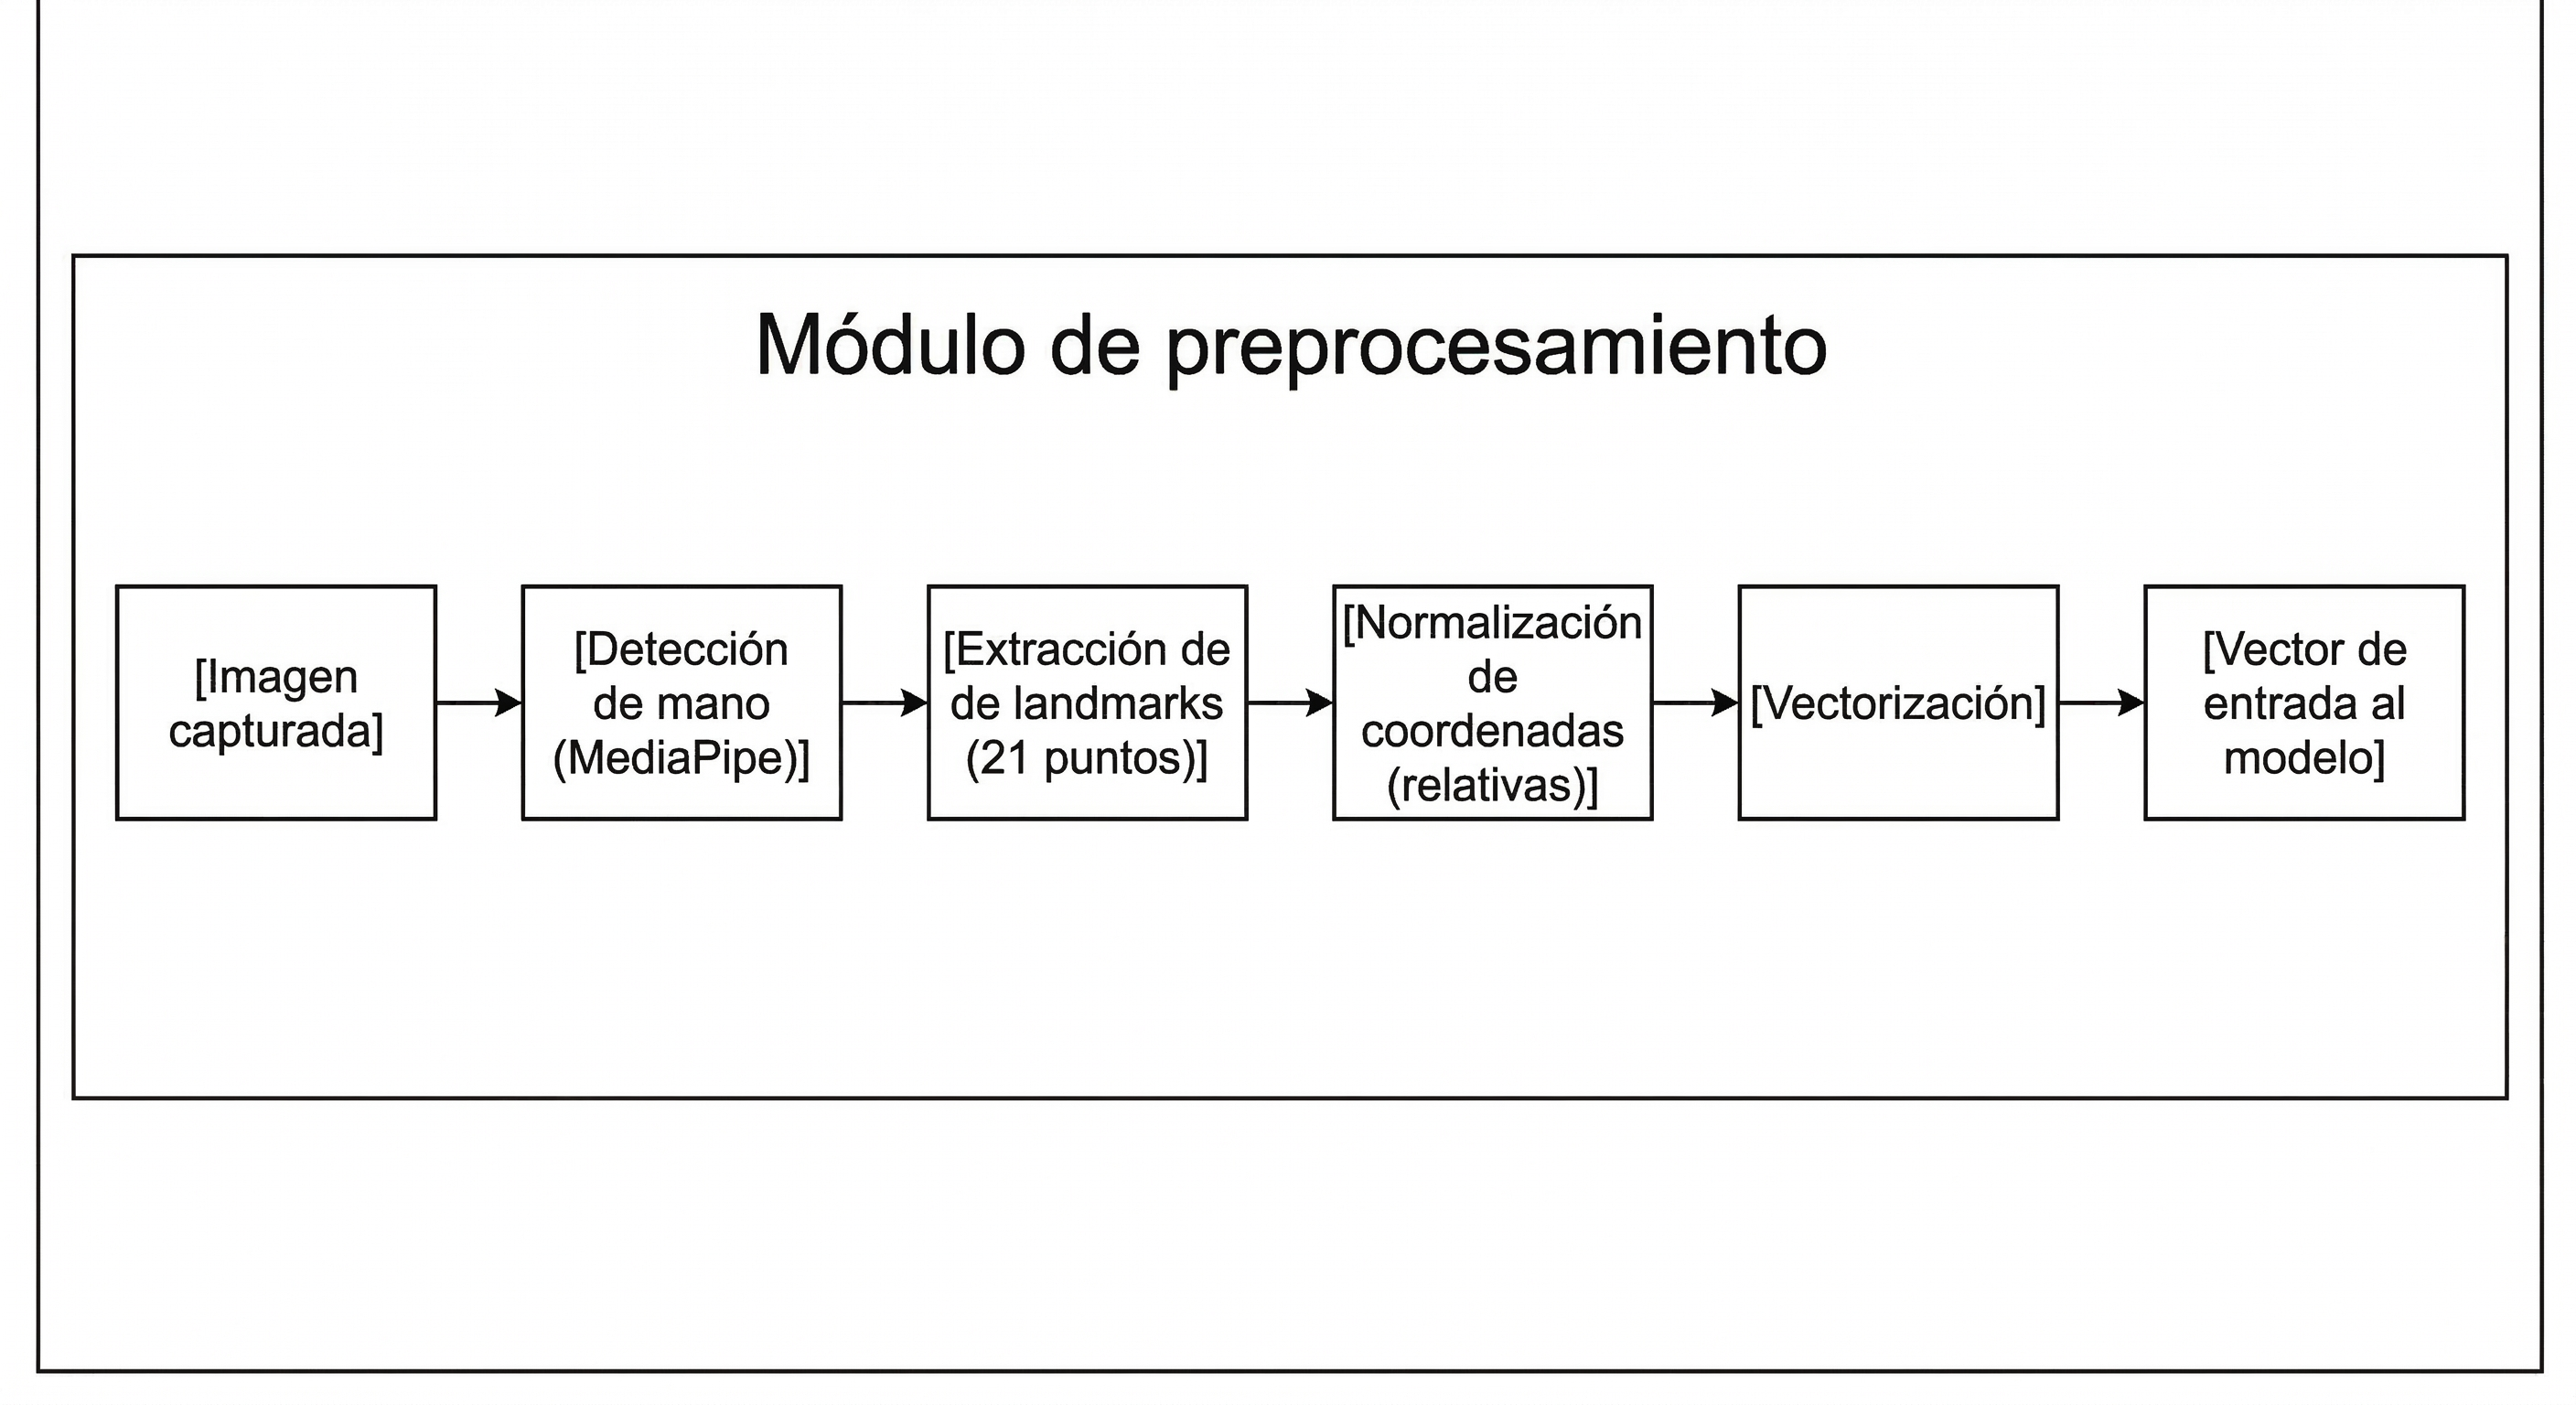
\includegraphics[width=0.6\textwidth]{images/fig31.png}
		\caption{Modulo de preprocesamiento.}
		\label{fig:mod_prepro}
	\end{figure}
	
	\textbf{Módulo de inferencia.}  
	
	Es el encargado de ejecutar el modelo de inteligencia artificial optimizado para su funcionamiento en dispositivos móviles mediante TensorFlow Lite. Este módulo recibe como entrada el vector de características generado en la etapa de preprocesamiento y produce como salida la clase correspondiente a la seña reconocida.
	
	Sus funciones principales incluyen:
	\begin{itemize}
		\item Cargar el modelo previamente entrenado y convertido a formato TensorFlow Lite.
		\item Ejecutar inferencias sobre los vectores de entrada generados a partir de los landmarks.
		\item Calcular la distribución de probabilidades de las clases mediante una función Softmax.
		\item Seleccionar la clase con mayor probabilidad como resultado final.
		\item Registrar métricas internas como latencia, uso de memoria y estabilidad del sistema.
	\end{itemize}
	
	El módulo de clasificación representa el núcleo del prototipo, ya que es responsable de transformar la representación numérica de la mano en una predicción semántica interpretable. A diferencia de enfoques tradicionales basados en redes convolucionales aplicadas directamente sobre imágenes, en este sistema el modelo opera sobre vectores de características derivados de landmarks, lo que reduce significativamente la complejidad computacional y permite su ejecución eficiente en dispositivos móviles.
	
	El modelo utilizado corresponde a una red neuronal ligera, como un perceptrón multicapa (MLP), adecuada para trabajar con datos estructurados. Este tipo de arquitectura permite aprender relaciones no lineales entre las coordenadas de los puntos clave de la mano, facilitando la discriminación entre diferentes señas.
	
	El modelo ha sido previamente convertido a formato TensorFlow Lite, lo cual permite su ejecución optimizada en CPU móviles, así como en aceleradores disponibles como GPU o NNAPI. De acuerdo con la documentación oficial, TensorFlow Lite está diseñado para reducir la latencia, el tamaño del modelo y el consumo energético, permitiendo inferencia continua en dispositivos con recursos limitados \cite{tflite}.
	
	En el proceso de clasificación el vector de entrada es procesado por la red neuronal, generando un vector de salida que representa las probabilidades asociadas a cada clase. Este vector es obtenido mediante una capa Softmax, la cual transforma la salida del modelo en una distribución de probabilidad \cite{softmax}. La clase con mayor probabilidad es seleccionada como la predicción final del sistema.
	
	La eficiencia de este módulo depende tanto del modelo como del hardware disponible. TensorFlow Lite permite optimizar el rendimiento mediante técnicas como cuantización y uso de delegados de hardware, lo que contribuye a reducir la latencia de inferencia \cite{tflite}.
	
	Como último paso el resultado generado corresponde a la etiqueta de la seña reconocida, acompañada opcionalmente de su probabilidad. Este resultado es enviado al módulo de visualización, donde se presenta al usuario en forma de texto.
	
	En consecuencia, el diseño del módulo de inferencia se orienta a garantizar una clasificación rápida, precisa y eficiente, manteniendo coherencia con el modelo entrenado y asegurando su viabilidad en un entorno móvil.
	
	\begin{figure}[H]
		\centering
		\begin{tikzpicture}[
			box/.style={
				draw,
				rectangle,
				minimum width=3.2cm,
				minimum height=1cm,
				align=center
			},
			myarrow/.style={
				-{Latex[length=3mm]},
				thick
			}
			]
			
			\node[box] (input) {Vector de entrada};
			\node[box, right=1cm of input] (model) {Modelo MLP\\(TFLite)};
			\node[box, right=1cm of model] (softmax) {Softmax};
			\node[box, right=1cm of softmax] (output) {Clase predicha};
			
			\draw[myarrow] (input) -- (model);
			\draw[myarrow] (model) -- (softmax);
			\draw[myarrow] (softmax) -- (output);
			
		\end{tikzpicture}
		\caption{Diagrama del módulo de inferencia del sistema.}
		\label{fig:inferencia}
	\end{figure}
	
	\textbf{Módulo de visualización.}  
	
	Se encarga de presentar al usuario el resultado final del proceso de reconocimiento y de proporcionar los elementos básicos de interacción con el sistema. Entre sus funciones principales se encuentran:
	\begin{itemize}
		\item Visualización del texto correspondiente a la seña reconocida.
		\item Retroalimentación visual inmediata del resultado.
		\item Botones para repetir el proceso o regresar a la vista de cámara.
		\item Indicadores de rendimiento en modo de depuración, tales como FPS, latencia y tamaño del modelo.
	\end{itemize}
	
	El módulo de visualización representa la etapa final del flujo de reconocimiento y es responsable de presentar al usuario el resultado obtenido por el modelo de clasificación. Aunque se trata de la última etapa del sistema, su función es crítica, ya que permite transformar la salida numérica generada por el modelo en una representación comprensible para el usuario. De acuerdo con principios de usabilidad en interfaces, la presentación del resultado debe ser inmediata, clara y libre de ambigüedad, manteniendo una comunicación directa entre el sistema y el usuario \cite{nng_heuristics}.
	
	Cuando el módulo de inferencia genera el vector de probabilidades, la clase con mayor valor es identificada como la predicción final. Sin embargo, esta salida se encuentra inicialmente en forma de un índice numérico asociado al orden de las clases definido durante el entrenamiento. Por ello, el módulo de visualización implementa un proceso de mapeo semántico, en el cual el índice predicho se transforma en la etiqueta textual correspondiente, por ejemplo, la letra o seña reconocida. TensorFlow Lite recomienda acompañar el modelo con un archivo de etiquetas para realizar esta conversión de manera consistente y evitar discrepancias entre índices y clases \cite{tflite}.
	
	El texto resultante debe desplegarse de forma clara en la interfaz. Para ello, el diseño del módulo considera principios de diseño visual para aplicaciones móviles, priorizando la legibilidad, el contraste y la jerarquía visual. Bajo estas recomendaciones, el resultado de la seña interpretada se muestra como texto central y de tamaño suficiente para facilitar su lectura de manera rápida \cite{material_design}.
	
	Además de mostrar la predicción, este módulo cumple una función de retroalimentación dentro del sistema. En aplicaciones interactivas, el usuario debe recibir una confirmación inmediata de que su acción fue procesada, evitando estados ambiguos o silenciosos \cite{nng_heuristics}. La visualización rápida del resultado permite confirmar que la captura, el procesamiento y la inferencia fueron ejecutados correctamente.
	
	El módulo de visualización se integra de manera fluida con el ciclo general de operación del sistema. Una vez mostrado el resultado, el usuario puede iniciar un nuevo proceso de reconocimiento o regresar a la vista principal de cámara. Así el diseño del módulo busca mantener una experiencia de uso clara, accesible y coherente con los principios de interacción móvil moderna \cite{material_design}.
	
	\begin{figure}[H]
		\centering
		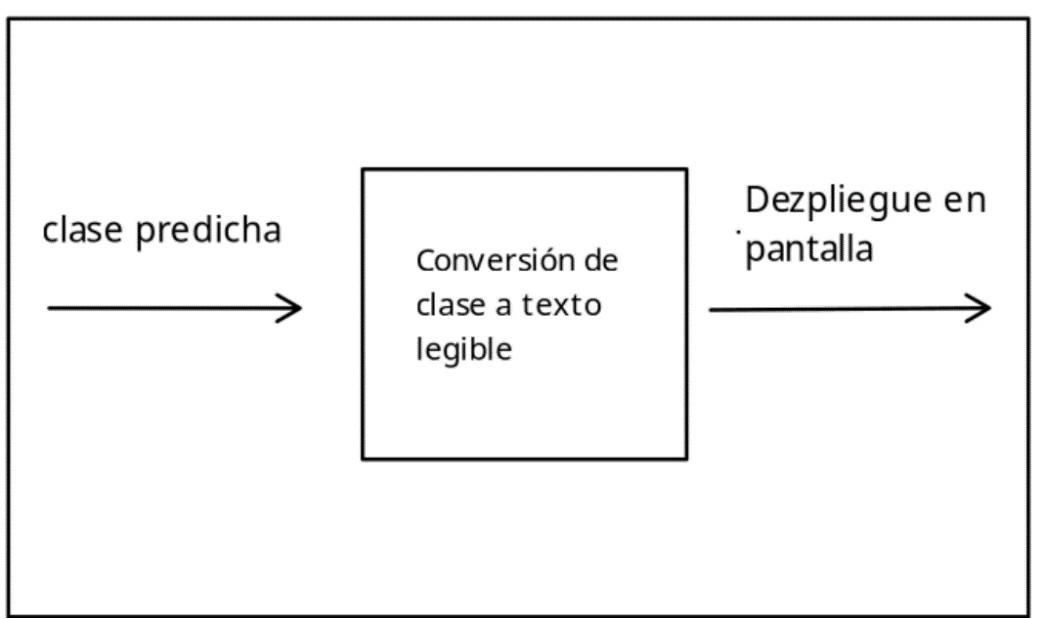
\includegraphics[width=0.6\textwidth]{images/fig32.jpg}
		\caption{Módulo de visualización de resultado.}
		\label{fig:Mod_vis}
	\end{figure}
	
	
	\subsection{Diseño de modelos}
	
	El diseño de modelos define la estrategia mediante la cual se construirá, entrenará, validará y seleccionará el modelo de aprendizaje automático encargado del reconocimiento de señas. Esta sección establece los lineamientos técnicos que guían la implementación del prototipo, asegurando coherencia entre las etapas de adquisición de datos, preprocesamiento, entrenamiento e inferencia.
	
	A diferencia de enfoques tradicionales basados en el uso de imágenes completas y redes neuronales convolucionales (CNN), el sistema propuesto adopta un enfoque basado en la extracción de características estructurales mediante landmarks. Esta decisión permite reducir significativamente la dimensionalidad del problema, disminuir el costo computacional y facilitar la ejecución del modelo en dispositivos móviles.
	
	Así el modelo no opera directamente sobre imágenes, sino sobre vectores de características derivados de la posición de puntos clave de la mano. Esto transforma el problema de reconocimiento visual en un problema de clasificación sobre datos estructurados.
	
	Los objetivos de esta sección son:
	\begin{itemize}
		\item Definir el proceso de transformación de datos desde imágenes hasta vectores de características.
		\item Establecer los modelos de clasificación candidatos.
		\item Determinar la configuración de entrenamiento y los hiperparámetros.
		\item Definir los métodos de validación y métricas de evaluación.
		\item Describir el proceso de integración del modelo en la aplicación móvil.
	\end{itemize}
	
	
	\subsubsection{Preprocesamiento}
	
	El preprocesamiento se encarga de transformar la información visual capturada en una representación numérica adecuada para el entrenamiento del modelo. En este prototipo el preprocesamiento se basa en la extracción de landmarks utilizando MediaPipe Hands, lo cual permite representar la geometría de la mano mediante un conjunto reducido de puntos clave.
	
	Cada muestra del dataset se procesa de la siguiente manera:
	
	\begin{itemize}
		\item Detección de la mano mediante MediaPipe.
		\item Extracción de 21 puntos clave (landmarks).
		\item Obtención de coordenadas espaciales $(x, y)$ por cada punto.
	\end{itemize}
	
	Esto da lugar a un vector inicial de 42 características por muestra.
	
	Posteriormente, se aplica un proceso de normalización de coordenadas con la finalidad de reducir la variabilidad asociada a la posición de la mano en la imagen. Para ello, se transforman las coordenadas a un sistema relativo, tomando como referencia un punto base o el valor mínimo en los ejes.
	
	Al final las coordenadas normalizadas se organizan en un vector unidimensional que será utilizado como entrada para el modelo de clasificación.
	
	Este enfoque presenta ventajas significativas:
	\begin{itemize}
		\item Reducción de dimensionalidad respecto a imágenes completas.
		\item Menor sensibilidad a condiciones de iluminación y fondo.
		\item Mayor eficiencia computacional.
	\end{itemize}
	
	\subsubsection{Modelos de clasificación}
	
	El problema abordado corresponde a una tarea de clasificación multiclase,
	 donde cada clase representa una seña del alfabeto en LSM.
	
	Dado que los datos de entrada corresponderán a vectores numéricos estructurados, se seleccionaran modelos de aprendizaje automático adecuados para este tipo de representación. Se consideran los siguientes modelos candidatos:
	
	\begin{itemize}
		\item Perceptrón multicapa (MLP)
		\item Máquinas de soporte vectorial (SVM)
		\item Bosques aleatorios (Random Forest)
	\end{itemize}
	
	El modelo principal seleccionado es el perceptrón multicapa (MLP), debido a su capacidad para modelar relaciones no lineales entre características y su compatibilidad con TensorFlow Lite para ejecución en dispositivos móviles.
	
	Las SVM y Random Forest se utilizan como modelos comparativos durante 
	la fase experimental destinados a evaluar el desempeño relativo del MLP.
	
	La selección final del modelo se realizará considerando:
	\begin{itemize}
		\item Precisión de clasificación
		\item Estabilidad del modelo
		\item Complejidad computacional
		\item Compatibilidad con despliegue móvil
	\end{itemize}
	
	\subsubsection{Hiperparámetros y entrenamiento}
	
	El entrenamiento del modelo se realizará utilizando un conjunto de datos
	previamente etiquetado. Para garantizar condiciones controladas, se establecerán configuraciones consistentes entre experimentos.
	
	Para el modelo MLP se considerarán los siguientes parámetros:
	
	\begin{itemize}
		\item Número de capas ocultas: 1 a 3
		\item Número de neuronas por capa: 64, 128 o 256
		\item Función de activación: ReLU
		\item Función de salida: Softmax
		\item Función de pérdida: CrossEntropy
		\item Optimizador: Adam
		\item Tasa de aprendizaje inicial: $10^{-3}$
		\item Número de épocas: 20 a 50
		\item Tamaño de lote (batch size): 16 a 32
	\end{itemize}
	
	Se incorporarán mecanismos de control para mejorar la estabilidad del entrenamiento:
	
	\begin{itemize}
		\item Early stopping para evitar sobreajuste
		\item Reducción de la tasa de aprendizaje en caso de estancamiento
		\item Uso de semillas fijas para reproducibilidad
	\end{itemize}
	\subsubsection{Validación}
	
	La evaluación del modelo se realizará mediante un esquema de validación 
	supervisada. Se utilizará una división del dataset en conjuntos de entrenamiento y prueba, así como validación cruzada para analizar la estabilidad del modelo.
	
	Las métricas de evaluación consideradas son:
	
	\begin{itemize}
		\item Accuracy
		\item Precision
		\item Recall
		\item F1-score
	\end{itemize}
	
	También se empleará la matriz de confusión para intentar identificar 
	patrones de error y evaluar la capacidad del modelo para distinguir entre clases similares.
	
	Estos métodos permitirán determinar el desempeño del modelo en términos de precisión y generalización.
	\subsubsection{Integración del modelo en Android}
	
	Después de seleccionar el modelo, se procederá a su conversión al formato TensorFlow Lite para su integración en la aplicación Android.
	
	Este proceso incluye:
	
	\begin{itemize}
		\item Exportación del modelo entrenado
		\item Conversión a formato TFLite
		\item Validación de consistencia entre entrenamiento e inferencia
	\end{itemize}
	
	El modelo será ejecutado directamente en el dispositivo móvil, permitiendo clasificación continua sin necesidad de conexión a internet.
	
	Por último se evaluará el desempeño del modelo en el entorno móvil mediante métricas como:
	
	\begin{itemize}
		\item Latencia de inferencia
		\item Uso de memoria
		\item Estabilidad
	\end{itemize}
	
	\subsection{Diseño de la interfaz gráfica del usuario}
	
	\subsubsection{Objetivos del diseño}
	
	El diseño de la interfaz gráfica del usuario tiene como propósito 
	principal facilitar la interacción entre el usuario y el sistema reconocimiento de señas, garantizando una experiencia de uso clara, eficiente y accesible. En este sentido, los objetivos del diseño se definen en función de los requerimientos funcionales del sistema, así como de las características del usuario objetivo.
	
	En primer lugar, se busca \textbf{proporcionar una interacción intuitiva 
	y de bajo esfuerzo cognitivo}, de modo que cualquier usuario, independientemente de su nivel de experiencia tecnológica, pueda utilizar la aplicación sin necesidad de capacitación previa. Esto implica minimizar la cantidad de acciones necesarias para ejecutar las funciones principales del sistema.
	
	Se establece como objetivo \textbf{garantizar la claridad en la 
	presentación de resultados}, mostrando de manera inmediata y comprensible la seña reconocida, junto con indicadores que permitan al usuario interpretar el nivel de confianza del sistema.
	
	Otro objetivo fundamental consiste en \textbf{ofrecer retroalimentación 
	visual}, permitiendo al usuario identificar cuándo el sistema está procesando información, cuándo una seña ha sido detectada correctamente y cuándo no existe una detección válida. Esto contribuye a mejorar la interacción y a reducir la incertidumbre durante el uso.
	
	También se busca \textbf{optimizar el flujo de interacción}, 
	reduciendo el número de pasos requeridos para iniciar el reconocimiento y obtener resultados, con el fin de favorecer un uso ágil y continuo del sistema.
	
	El diseño persigue \textbf{mantener consistencia visual y
	funcional en todas las pantallas}, asegurando que los elementos de la interfaz conserven un comportamiento predecible y homogéneo, lo cual mejora la usabilidad general del sistema.
	
	Finalmente se plantea como objetivo \textbf{soportar la evaluación de 
	usabilidad del sistema}, incorporando elementos medibles como tiempos de respuesta, número de interacciones y claridad de la información presentada, lo que permitirá validar la calidad de la interfaz en etapas posteriores del proyecto.
	
	\subsubsection{Principios de diseño}
	
	El diseño de la interfaz gráfica del sistema se desarrolló considerando principios
	de usabilidad y diseño de interfaces humano-computadora orientados a dispositivos
	móviles. Estos principios permiten estructurar interfaces más comprensibles,
	consistentes y eficientes para el usuario en la interacción con el sistema
	\cite{nielsen1994usability,shneiderman2016designing,norman2013design}.
	
	Uno de los criterios principales fue reducir la cantidad de elementos visuales
	presentes en pantalla en el proceso de reconocimiento. De acuerdo con Nielsen
	\cite{nielsen1994usability}, una interfaz con exceso de información puede aumentar
	la carga cognitiva del usuario y dificultar la identificación de las funciones
	principales del sistema. Por esta razón, la interfaz del prototipo mantiene visibles
	únicamente los componentes necesarios para la operación del reconocimiento, tales
	como el área de captura, los controles principales y la visualización del resultado
	obtenido.
	
	Se aplicó el principio de consistencia visual y funcional, manteniendo
	la misma distribución de elementos, estilos gráficos y comportamiento de navegación
	entre las distintas pantallas de la aplicación. Shneiderman
	\cite{shneiderman2016designing} establece que la consistencia en interfaces reduce
	la curva de aprendizaje y permite que los usuarios comprendan con mayor facilidad
	el funcionamiento general del sistema.
	
	También se incorporaron mecanismos de retroalimentación visual para informar al
	usuario sobre el estado actual del reconocimiento. Norman
	\cite{norman2013design} menciona que la retroalimentación inmediata constituye uno
	de los principios fundamentales del diseño interactivo, ya que permite al usuario
	comprender las acciones ejecutadas por el sistema y verificar que el proceso se
	está realizando correctamente. En el prototipo desarrollado, esta retroalimentación
	se presenta mediante la visualización de la seña detectada, indicadores de captura
	y actualización continua de los resultados generados por el modelo de clasificación.
	
	Otro aspecto considerado fue la reducción de interacciones necesarias para acceder
	a las funciones principales de la aplicación. Según Pressman
	\cite{pressman2014software}, los sistemas orientados a la interacción continua
	deben minimizar operaciones innecesarias para mejorar la eficiencia de uso y
	disminuir posibles errores de operación. Por ello, las funciones principales del
	sistema fueron organizadas de manera jerárquica y accesible desde las pantallas
	principales de la aplicación.
	
	El diseño contempló criterios relacionados con accesibilidad visual
	en dispositivos móviles. Sommerville \cite{sommerville2016software} señala que las
	interfaces deben considerar aspectos como legibilidad, contraste y tamaño adecuado
	de los componentes gráficos para facilitar la interacción en distintos entornos de
	uso. En consecuencia, se emplearon tamaños de texto legibles, botones con áreas de
	interacción adecuadas y contrastes visuales que permiten distinguir claramente los
	distintos elementos presentes en pantalla.
	
	Finalmente el diseño de la interfaz fue orientado a mantener un flujo de
	interacción continuo entre el usuario y el sistema de reconocimiento, 
	procurando
	que los elementos principales puedan ser identificados rápidamente durante el uso
	de la aplicación móvil.
	
	
	\subsubsection{Estructura general de la aplicación}
	
	La aplicación móvil desarrollada fue estructurada bajo un esquema modular,
	permitiendo separar las funciones relacionadas con autenticación, navegación,
	reconocimiento de señas y configuración del sistema. La organización general de
	la aplicación busca facilitar el acceso a las funciones principales mediante un
	flujo de navegación continuo y jerárquico.
	
	El flujo principal de la aplicación inicia con la pantalla de carga
	(\textit{Splash Screen}), seguida del proceso de autenticación y aceptación de
	términos de uso y aviso de privacidad. Posteriormente, el usuario accede al menú
	principal, desde el cual puede navegar hacia los distintos módulos disponibles
	dentro del sistema.
	
	Entre los módulos principales se encuentran el intérprete de señas, el
	diccionario de apoyo, el historial de detecciones y las opciones de configuración
	del perfil. El módulo de reconocimiento es la función central de la
	aplicación, ya que permite capturar imágenes mediante la cámara frontal del
	dispositivo y ejecutar el proceso de reconocimiento de señas utilizando el modelo
	de clasificación implementado localmente en el dispositivo móvil.
	
	El sistema incorpora un flujo interno de procesamiento compuesto por la
	captura de imágenes, detección de puntos clave de la mano mediante MediaPipe
	Hands, generación del vector de características y clasificación utilizando
	TensorFlow Lite. Como último paso los resultados obtenidos son mostrados dentro de la
	interfaz gráfica de la aplicación.
	
	La Figura~\ref{fig:flujo_general_app} muestra el flujo general de navegación y la
	estructura principal de módulos implementados dentro de la aplicación móvil
	desarrollada.
	
	\begin{figure}[H]
		\centering
		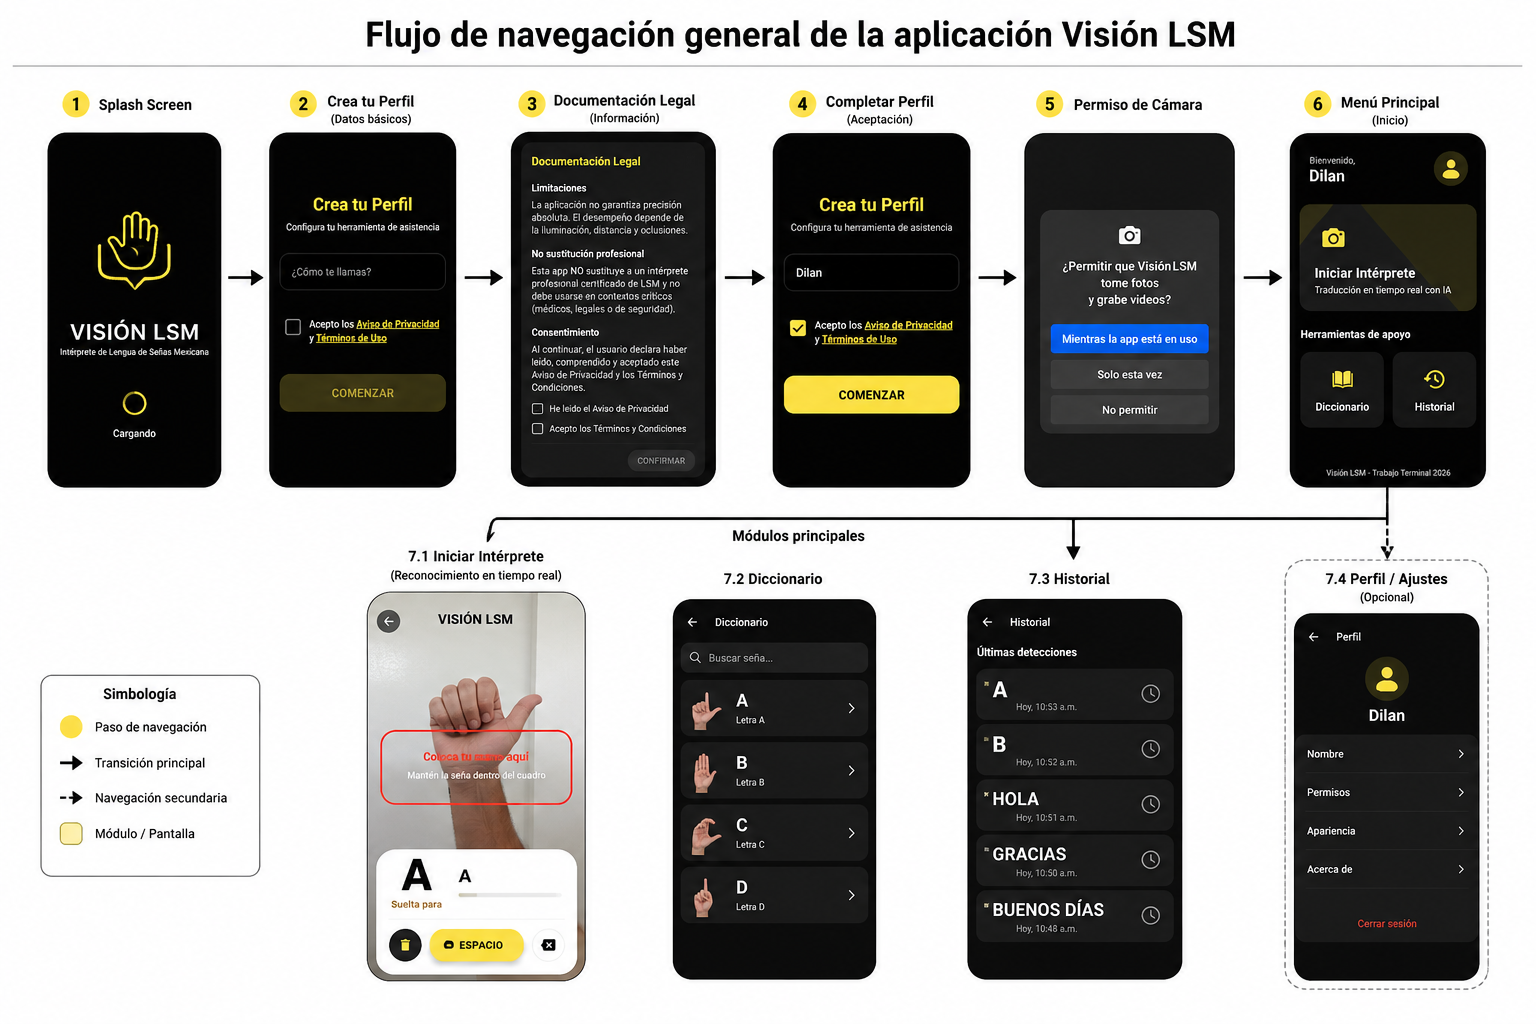
\includegraphics[width=1\textwidth]{images/fig36.png}
		\caption{Módulo de visualización de resultado.}
		\label{fig:flujo_general_app}
	\end{figure}
		
	\subsubsection{Diseño de pantallas principales}
	
	El diseño de las pantallas principales de la aplicación fue desarrollado
	considerando criterios de organización funcional, accesibilidad visual y
	consistencia de navegación dentro del entorno móvil. Cada pantalla fue diseñada
	con un propósito específico dentro del flujo general de interacción, buscando
	mantener una distribución clara de los elementos y reducir la cantidad de acciones
	necesarias para acceder a las funciones principales del sistema.
	
	De acuerdo con Shneiderman \cite{shneiderman2016designing}, una correcta
	organización de interfaces permite mejorar la comprensión del sistema y facilitar
	la navegación entre módulos relacionados. Nielsen
	\cite{nielsen1994usability} establece que las interfaces deben mantener
	consistencia visual y funcional para reducir errores de interacción y mejorar el
	aprendizaje del usuario en el uso de la aplicación.
	
	Las pantallas desarrolladas dentro del prototipo fueron organizadas de acuerdo con
	las funciones principales del sistema, incluyendo módulos de autenticación,
	navegación principal, reconocimiento de señas y herramientas complementarias de
	apoyo. A continuación, se describen las principales pantallas implementadas dentro
	de la aplicación móvil desarrollada.
	
	\paragraph{Pantalla de inicio y autenticación}
	
	
	La pantalla de inicio y autenticación concentra el primer punto de interacción
	entre el usuario y la aplicación. Su propósito es registrar un identificador
	básico del usuario, presentar la documentación legal correspondiente y solicitar
	la aceptación explícita del aviso de privacidad y los términos de uso antes de
	permitir el acceso a las funciones principales del sistema.
	
	Desde el punto de vista de usabilidad, esta pantalla incorpora validación de
	entrada y control de estados. En el estado inicial, el botón de acceso permanece
	deshabilitado mientras el usuario no ingrese su nombre y no acepte la
	documentación correspondiente. Esta decisión se relaciona con el principio de
	prevención de errores, el cual establece que una interfaz debe evitar que el
	usuario ejecute acciones inválidas o incompletas antes de continuar con el flujo
	del sistema \cite{nielsen1994usability}. Una vez completados los datos mínimos
	requeridos, la interfaz habilita el botón de inicio, proporcionando una señal
	visual clara de que el usuario puede avanzar al menú principal.
	
	La pantalla también incorpora un modal de documentación legal, donde se presentan
	las limitaciones del prototipo, la aclaración de que la aplicación no sustituye a
	un intérprete profesional certificado de LSM y las condiciones de consentimiento.
	Este mecanismo permite separar la información legal del formulario principal,
	evitando saturar visualmente la pantalla inicial y manteniendo disponible la
	información relevante antes de la aceptación del usuario.
	
	Debido a que el sistema utiliza la cámara del dispositivo móvil para capturar
	imágenes de la mano durante el proceso de reconocimiento, se consideraron aspectos
	relacionados con privacidad y protección de datos personales. La Ley Federal de
	Protección de Datos Personales en Posesión de los Particulares establece que el
	tratamiento de datos personales debe realizarse de forma legítima, controlada e
	informada, garantizando la privacidad y el derecho a la autodeterminación
	informativa de las personas \cite{lfpdppp}. La guía sobre datos
	biométricos publicada por el INAI señala que este tipo de información debe
	tratarse atendiendo principios de protección de datos personales, en particular
	cuando permite identificar o hacer identificable a una persona \cite{inaiBiometricos}.
	
	En este prototipo, las imágenes capturadas por la cámara no se almacenan ni se
	envían a servidores externos. El procesamiento se realiza localmente en el
	dispositivo móvil y las imágenes se utilizan únicamente como entrada temporal para
	la detección de landmarks, el preprocesamiento y la inferencia del modelo. Esta
	decisión reduce el tratamiento de información visual sensible, evita la creación
	de bases de datos de imágenes o video de los usuarios y disminuye los riesgos
	asociados a la transmisión de información personal.
	
	La Figura~\ref{fig:autenticacion_estados} muestra los principales estados de la
	pantalla de autenticación: el formulario inicial, la documentación legal y el
	estado final con los datos requeridos completados.
	
	
	\begin{figure}[H]
		\centering
		
\includegraphics[width=0.32\textwidth]{images/fig37.jpg}
		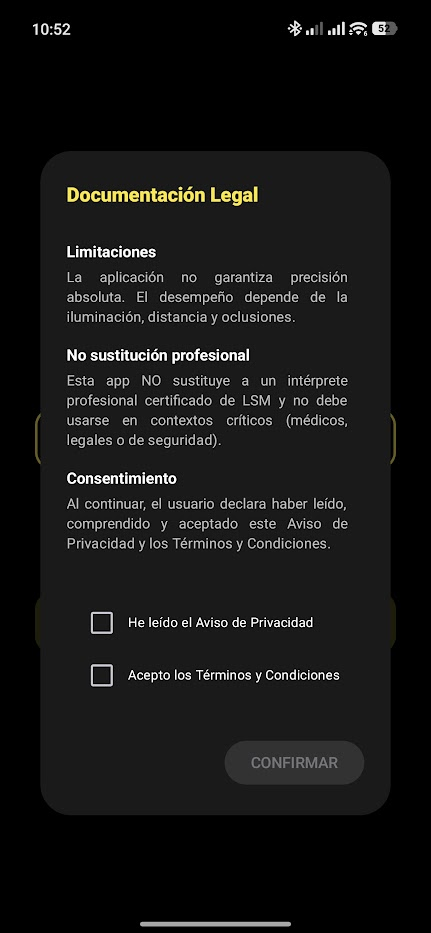
\includegraphics[width=0.32\textwidth]{images/fig38.jpg}
		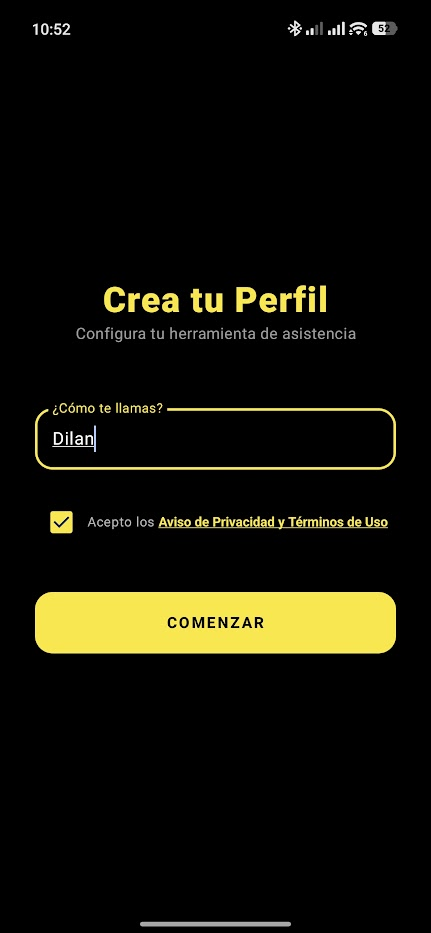
\includegraphics[width=0.32\textwidth]{images/fig39.jpg}
		\caption{Estados principales de la pantalla de autenticación y consentimiento:
			(a) formulario inicial, (b) documentación legal y (c) validación de datos para
			acceso al sistema.}
		\label{fig:autenticacion_estados}
	\end{figure}
	
	\paragraph{Pantalla principal}
	
	La pantalla principal funciona como el punto central de navegación dentro de la
	aplicación móvil. Su propósito es permitir al usuario acceder de manera organizada
	a las funcionalidades principales del sistema, incluyendo el módulo de
	reconocimiento de señas, el diccionario de apoyo, el historial de detecciones y
	las opciones relacionadas con el perfil del usuario.
	
	La distribución de los componentes dentro de esta pantalla fue diseñada siguiendo
	criterios de jerarquía visual y organización funcional. De acuerdo con
	Shneiderman \cite{shneiderman2016designing}, una adecuada organización visual
	permite que los usuarios identifiquen con mayor rapidez las funciones principales
	del sistema y reduzcan el tiempo necesario para navegar entre distintos módulos.
	Por esta razón, el acceso al intérprete de señas se presenta como el componente
	visual predominante dentro de la interfaz, destacando la funcionalidad principal
	del prototipo.
	
	Las herramientas complementarias, como el diccionario y el historial,
	fueron agrupadas en una sección independiente con la finalidad de mantener una
	separación clara entre las funciones principales y secundarias del sistema. Esta
	organización contribuye a mantener una navegación más estructurada y facilita la
	identificación de cada módulo disponible dentro de la aplicación.
	
	Desde el punto de vista visual, la pantalla mantiene consistencia respecto al uso
	de colores, tipografía y distribución de elementos implementados en el resto de
	la aplicación. Nielsen \cite{nielsen1994usability} establece que la consistencia
	en interfaces reduce errores de interacción y mejora la comprensión general del
	sistema por parte del usuario.
	
	La Figura~\ref{fig:pantalla_principal} muestra la pantalla principal implementada
	dentro de la aplicación móvil desarrollada.
	
	\begin{figure}[H]
		\centering
		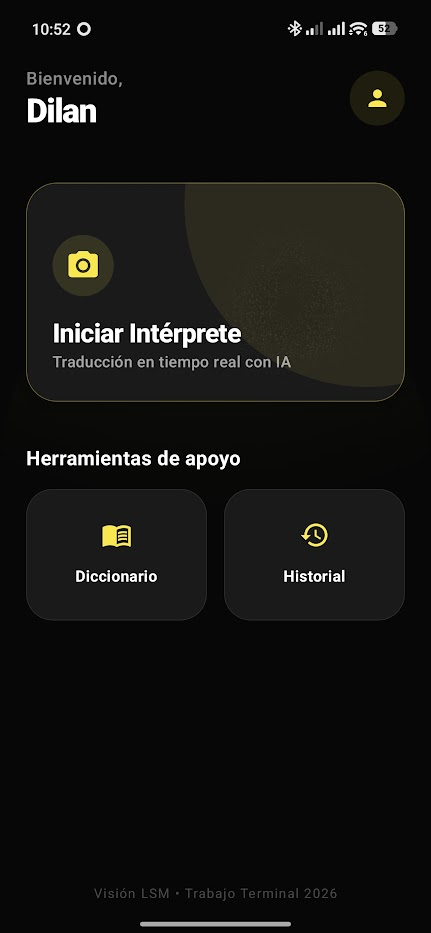
\includegraphics[width=0.33\textwidth]{images/fig40.jpg}
		\caption{Pantalla principal de la aplicación VisiónLSM.}
		\label{fig:pantalla_principal}
	\end{figure}
	
		
	\paragraph{Pantalla de reconocimiento en señas}
	
	Esta pantalla fue diseñada para mantener visibles
	los elementos necesarios en la interacción del usuario con el sistema,
	permitiendo visualizar simultáneamente el área de captura, las indicaciones de
	uso y los resultados generados por el modelo de clasificación.
	
	Uno de los elementos principales de esta pantalla corresponde al área guía de
	captura, representada mediante un cuadro delimitador visible sobre la imagen de la
	cámara. Este elemento tiene como objetivo indicar al usuario la región recomendada
	para posicionar la mano en el proceso de reconocimiento. De acuerdo con
	Norman \cite{norman2013design}, las interfaces deben proporcionar señales visuales
	claras que orienten al usuario sobre cómo interactuar correctamente con el
	sistema. En este caso, el cuadro de captura funciona como un mecanismo de apoyo
	visual para mejorar la interacción con el módulo de reconocimiento.
	
	La interfaz incorpora mensajes de estado relacionados con el uso de la
	cámara y el proceso de detección. Cuando el sistema no cuenta con permisos de
	acceso a la cámara, se presenta una notificación visual indicando la necesidad de
	habilitar dicho permiso para utilizar las funciones de reconocimiento. Esta medida
	permite mantener informado al usuario sobre el estado actual del sistema y evitar
	fallos derivados de permisos no concedidos.
	
	Cuando se habilite la cámara, la pantalla muestra el resultado del proceso de
	clasificación mediante la visualización de la letra detectada y un indicador
	gráfico asociado al nivel de confianza generado por el modelo. Nielsen
	\cite{nielsen1994usability} establece que los sistemas interactivos deben ofrecer
	retroalimentación continua acerca de las acciones realizadas y del estado actual
	del sistema. En consecuencia, el prototipo desarrollado actualiza visualmente los
	resultados obtenidos en el reconocimiento continuo de señas.
	
	La interfaz incorpora botones de interacción rápida destinados a
	la gestión del texto reconocido. Entre estas funciones se incluyen opciones para
	eliminar caracteres detectados y agregar espacios dentro de la construcción de
	palabras o frases generadas mediante el reconocimiento de señas. Estas acciones
	permiten complementar el flujo de interacción entre el usuario y el sistema
	dur de interpretación.
	
	Desde el punto de vista visual, la pantalla mantiene consistencia con el resto de
	la aplicación mediante el uso de una paleta de colores basada en tonos oscuros y
	acentos amarillos. Asimismo, se utilizaron contrastes altos entre texto y fondo
	para favorecer la visibilidad de los elementos principales relacionados con el
	reconocimiento.
	
	La Figura~\ref{fig:reconocimiento_estados} muestra los principales estados de la
	pantalla de reconocimiento: la solicitud de permisos de cámara y el proceso
	activo de detección y clasificación de señas.
	
	\begin{figure}[H]
		\centering
		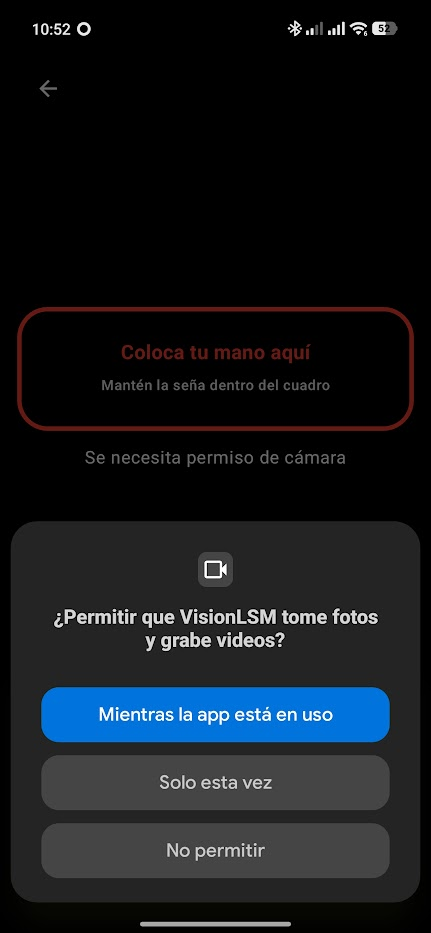
\includegraphics[width=0.30\textwidth]{images/fig41.jpg}
		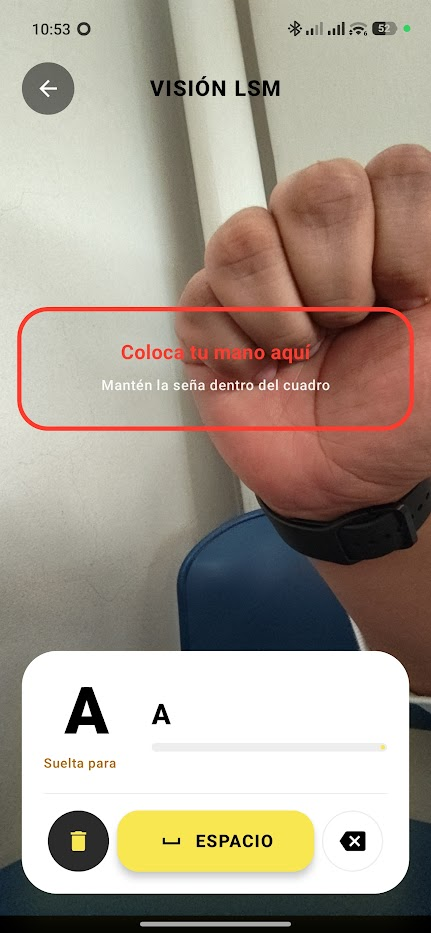
\includegraphics[width=0.30\textwidth]{images/fig42.jpg}
		\caption{Estados principales de la pantalla de reconocimiento:
			(a) solicitud de permisos de cámara y
			(b) proceso activo de reconocimiento de señas.}
		\label{fig:reconocimiento_estados}
	\end{figure}
	
		
	\paragraph{Pantallas complementarias}
	% Diccionario y configuración (puedes agruparlas)
	
	\subsubsection{Interacción del usuario}
	
	La interacción del usuario con la aplicación fue diseñada buscando reducir la
	cantidad de acciones necesarias para acceder a las funciones principales del
	sistema dentro del entorno móvil. La organización de navegación implementada
	permite que el usuario pueda acceder al módulo de reconocimiento de señas
	realizando una secuencia corta de interacciones desde la pantalla principal.
	
	El proceso de uso comienza con la carga inicial de la aplicación, seguida del
	registro de un identificador básico del usuario y la aceptación del aviso de
	privacidad y términos de uso. Una vez completado este proceso, el usuario accede
	al menú principal, donde el módulo de reconocimiento puede iniciarse mediante una
	única selección dentro de la interfaz.
	
	Durante el reconocimiento de señas, la interacción requerida por parte del usuario
	consiste principalmente en posicionar la mano dentro del área de captura mostrada
	en pantalla y utilizar controles específicos relacionados con la edición del texto
	detectado. Entre estos controles se incluyen botones para agregar espacios y
	eliminar caracteres reconocidos en la interpretación.
	
	De acuerdo con Nielsen \cite{nielsen1994usability}, la reducción de pasos
	innecesarios y la organización adecuada de las acciones principales contribuyen a
	disminuir errores de interacción dentro de sistemas interactivos.
	Shneiderman \cite{shneiderman2016designing} establece que las interfaces deben
	mantener una navegación consistente y permitir que las funciones principales sean
	identificadas rápidamente por el usuario.
	
	Las funciones principales de la aplicación fueron organizadas de
	forma jerárquica dentro del menú principal, priorizando el acceso al módulo de
	reconocimiento respecto a las herramientas complementarias del sistema.
	
	La aplicación incorpora mecanismos de retroalimentación visual que
	permiten informar continuamente al usuario sobre el estado actual de la aplicación.
	Entre estos mecanismos se incluyen mensajes relacionados con permisos de cámara,
	indicadores de detección de señas y actualización visual de los resultados
	obtenidos en el proceso de clasificación.
	
	También la interacción general del sistema fue diseñada considerando las
	restricciones propias de dispositivos móviles, utilizando botones con dimensiones
	adecuadas para interacción táctil, elementos de navegación visibles y una
	distribución organizada de los componentes principales dentro de cada pantalla de
	la aplicación.
	
	\subsubsection{Diseño visual}
	
	El diseño visual de la aplicación fue desarrollado considerando criterios de
	legibilidad, contraste, consistencia visual y diferenciación funcional de los
	elementos presentes dentro de la interfaz móvil. Estos criterios son importantes en aplicaciones de reconocimiento visual, donde el
	usuario debe identificar rápidamente información relacionada con la captura,
	detección y clasificación de señas.
	
	De acuerdo con la norma ISO 9241-110 \cite{iso9241}, los sistemas interactivos
	deben proporcionar una presentación clara de la información y mantener una
	consistencia visual que facilite la identificación de funciones y estados dentro
	de la interfaz. Asimismo, Material Design \cite{materialDesign} establece que la
	paleta de colores utilizada en aplicaciones móviles debe favorecer el contraste,
	la diferenciación jerárquica de componentes y la accesibilidad visual en la
	interacción del usuario.
	
	Considerando estos principios, el prototipo desarrollado contempla una interfaz
	basada en combinaciones de colores de alto contraste, principalmente mediante el
	uso de fondos oscuros o claros acompañados de colores de acento destinados a
	resaltar elementos interactivos y estados relevantes del sistema. Esta decisión
	busca mejorar la visibilidad de los componentes principales y facilitar la
	identificación rápida de funciones relacionadas con el reconocimiento de señas.
	
	Dentro de las propuestas visuales consideradas para la aplicación se encuentran
	dos variantes principales de interfaz: una basada en tema oscuro y otra basada en
	tema claro. La variante oscura utiliza fondos en tonos negros y grises oscuros
	acompañados de colores de acento en amarillo, mientras que la variante clara
	emplea fondos blancos o grises claros manteniendo los mismos elementos de acento.
	Ambas configuraciones permiten conservar consistencia visual entre pantallas y
	mantener diferenciación clara entre elementos activos, información principal y
	controles secundarios.
	
	Se contempló la incorporación de colores asociados a estados del
	sistema dentro del módulo de reconocimiento. Estos estados incluyen indicadores
	visuales para procesos como detección activa de señas, errores de captura,
	ausencia de permisos o resultados generados por el modelo de clasificación. El
	uso de colores diferenciados para estados funcionales permite proporcionar
	retroalimentación visual inmediata y facilita la interpretación del estado actual
	del sistema en la interacción con la aplicación.
	
	El diseño visual considera el uso consistente de tipografías,
	espaciado entre componentes y tamaños adecuados para interacción táctil en
	dispositivos móviles. Estas decisiones buscan mantener claridad visual dentro de
	la interfaz y mejorar la identificación de los elementos principales durante el
	uso del sistema.
	
	La propuesta visual implementada busca mantener coherencia estética y
	funcional entre todos los módulos de la aplicación, permitiendo que los usuarios
	identifiquen rápidamente las acciones principales y los estados asociados al
	proceso de reconocimiento de señas.

	
	\subsubsection{Evaluación de usabilidad}
	
	En el desarrollo del diseño de la interfaz gráfica del prototipo se consideraron distintos
	criterios relacionados con usabilidad dentro del entorno móvil. De acuerdo con la
	norma ISO 9241-11 \cite{iso9241usability}, la usabilidad se relaciona con la
	capacidad de un sistema para ser utilizado de forma efectiva y comprensible por
	determinados usuarios dentro de un contexto de uso específico.
	
	Considerando estos principios, la interfaz de la aplicación fue organizada
	buscando mantener visibilidad adecuada de las funciones principales, reducir la
	cantidad de acciones necesarias para acceder al módulo de reconocimiento y
	proporcionar retroalimentación visual en la interacción del usuario con el
	sistema.
	
	Se contemplaron aspectos relacionados con legibilidad, contraste visual,
	distribución de componentes y consistencia entre pantallas. Estos elementos fueron
	considerados con el objetivo de
	favorecer la identificación de los módulos principales del sistema.
	
	El diseño de la interfaz considera mecanismos visuales para
	informar al usuario sobre el estado actual del sistema, incluyendo mensajes
	relacionados con permisos de cámara, detección de señas y visualización de los
	resultados generados en la clasificación.
	
	Los criterios de usabilidad considerados en el diseño servirán
	como base para las pruebas funcionales y de interacción descritas posteriormente
	en el capítulo de implementación y evaluación del prototipo.
	
	
	\newpage
	

